%%%%%%%%%%%%%%%%%%%%%%% file template.tex %%%%%%%%%%%%%%%%%%%%%%%%%
%
% This is a general template file for the LaTeX package SVJour3
% for Springer journals.          Springer Heidelberg 2010/09/16
%
% Copy it to a new file with a new name and use it as the basis
% for your article. Delete % signs as needed.
%
% This template includes a few options for different layouts and
% content for various journals. Please consult a previous issue of
% your journal as needed.
%
%%%%%%%%%%%%%%%%%%%%%%%%%%%%%%%%%%%%%%%%%%%%%%%%%%%%%%%%%%%%%%%%%%%
%
\RequirePackage{fix-cm}
%
%\documentclass{svjour3}                     % onecolumn (standard format)
%\documentclass[smallcondensed]{svjour3}     % onecolumn (ditto)
\documentclass[smallextended]{svjour3}       % onecolumn (second format)
%\documentclass[twocolumn]{svjour3}          % twocolumn
%
\smartqed  % flush right qed marks, e.g. at end of proof
%
\usepackage{amsmath, amssymb}
\usepackage{graphicx}
\usepackage{amsfonts}
\usepackage{subcaption}
\usepackage{hyperref}
%\usepackage{pdflscape} % Landscape pages
\usepackage{color}	% Different font colors
\usepackage{enumerate}
\usepackage{enumitem}
\usepackage{mathtools}
\usepackage[]{algorithm2e}
\usepackage{color}
\usepackage{multirow} % Merging rows in tables
\usepackage{multicol} % Merging columns in tables
\usepackage{booktabs} % Horizontal rules in tables

\newcommand{\indentitem}{\setlength\itemindent{18pt}}
\renewcommand{\labelitemi}{$\bullet$}
\captionsetup{compatibility=false}
\newtheorem{prop}{Proposition}
\newtheorem{obs}{Observation}
\newtheorem{cor}{Corollary}
\newcommand\mycommfont[1]{\footnotesize\ttfamily\textcolor{blue}{#1}}
\SetCommentSty{mycommfont}
\SetKwRepeat{Do}{do}{while}
%
% \usepackage{mathptmx}      % use Times fonts if available on your TeX system
%
% insert here the call for the packages your document requires
%\usepackage{latexsym}
% etc.
%
% please place your own definitions here and don't use \def but
% \newcommand{}{} 
%
% Insert the name of "your journal" with
% \journalname{myjournal}
%
% original amsmath definition
% \subequations:
% \long macro:->\refstepcounter {equation}\protected@edef \theparentequation {\theequation }\setcounter {parentequation}{\value {equation}}\setcounter {equation}{0}\def \theequation {\theparentequation \alph {equation}}\ignorespaces 

% saved by hyperref in
% > \HyOrg@subequations=\long macro:

% hyperref-patched \subequations: (\endsubequations not modified)
% > \subequations=macro:
% ->\stepcounter {equation}\protected@edef \theHparentequation {\@ifundefined {th
% eHequation}\theequation \theHequation }\addtocounter {equation}{-1}\HyOrg@subeq
% uations \def \theHequation {\theHparentequation \alph {equation}}\ignorespaces 
% .


% extending the environment
%   1. with optional parameter: expected values resume or intermezzo or none.
%   2. while keeping the hyperref customization.

\makeatletter
\def\user@resume{resume}
\def\user@intermezzo{intermezzo}
%
\newcounter{previousequation}
\newcounter{lastsubequation}
\newcounter{savedparentequation}
\setcounter{savedparentequation}{1}
% 
% The following code causes that we are able to continue with numbering of a model in a next \align .
% For example:
%    a < b    (1a)
%    a < c    (1b)
% some text comes here and the numbering will continue:
%    a < d    (1c)
%
\renewenvironment{subequations}[1][]{%
      \def\user@decides{#1}%
      \setcounter{previousequation}{\value{equation}}%
      \ifx\user@decides\user@resume 
           \setcounter{equation}{\value{savedparentequation}}%
      \else  
      \ifx\user@decides\user@intermezzo
           \refstepcounter{equation}%
      \else
           \setcounter{lastsubequation}{0}%
           \refstepcounter{equation}%
      \fi\fi
      \protected@edef\theHparentequation{%
          \@ifundefined {theHequation}\theequation \theHequation}%
      \protected@edef\theparentequation{\theequation}%
      \setcounter{parentequation}{\value{equation}}%
      \ifx\user@decides\user@resume 
           \setcounter{equation}{\value{lastsubequation}}%
         \else
           \setcounter{equation}{0}%
      \fi
      \def\theequation  {\theparentequation  \alph{equation}}%
      \def\theHequation {\theHparentequation \alph{equation}}%
      \ignorespaces
}{%
%  \arabic{equation};\arabic{savedparentequation};\arabic{lastsubequation}
  \ifx\user@decides\user@resume
       \setcounter{lastsubequation}{\value{equation}}%
       \setcounter{equation}{\value{previousequation}}%
  \else
  \ifx\user@decides\user@intermezzo
       \setcounter{equation}{\value{parentequation}}%
  \else
       \setcounter{lastsubequation}{\value{equation}}%
       \setcounter{savedparentequation}{\value{parentequation}}%
       \setcounter{equation}{\value{parentequation}}%
  \fi\fi
%  \arabic{equation};\arabic{savedparentequation};\arabic{lastsubequation}
  \ignorespacesafterend
}
\makeatother

\begin{document}

\title{Comparison of Mixed Integer Programming Formulations for the Shared Multicast Tree Problem
%\thanks{Grants or other notes
%about the article that should go on the front page should be
%placed here. General acknowledgments should be placed at the end of the article.}
}
\subtitle{Tightening the LP bounds}
\titlerunning{Comparison of MIP formulations for SMT}        % if too long for running head

\author{Marika Ivanova        \and
         Dag Haugland
}
%\authorrunning{Short form of author list} % if too long for running head

\institute{F. Author \at
              first address \\
              Tel.: +123-45-678910\\
              Fax: +123-45-678910\\
              \email{fauthor@example.com}           %  \\
%             \emph{Present address:} of F. Author  %  if needed
           \and
           S. Author \at
              second address
}

\date{Received: date / Accepted: date}
% The correct dates will be entered by the editor
\maketitle

\begin{abstract}
In this paper we focus on the Shared Multicast Tree problem (SMT), which is 
a task in wireless network design aiming to establish a wireless 
communication network minimizing necessary energy consumption. SMT is a 
generalization of the Shared Broadcast Tree problem (SBT), and can be 
regarded as a Steiner tree problem with a nonlinear objective functinon that
reflects the use in wireless communication. In particular, we consider two 
integer linear programming formulations and investigate how they relate to 
each other.  Both models are subsequently extended by additional variables and corresponding constraints. We also present several valid inequalities. Our goal is to achieve a stronger LP bound than models studied in previous works, and also to devise 
a method which allows computing these lower bounds for instances as 
large as possible. Numerical experiments suggest that both models are much 
stronger than previous formulations, however, the number of constraints 
makes them impractical for solving instances of even fairly small size as 
the computation takes prohibitively long time. Applying a constraint 
generation scheme on one of the studied models substantially increases the 
size of the instances for which it is possible to obtain a strong LP 
bound. 
\keywords{Wireless communication, broadcast tree, multicast, Steiner tree, LP bound, 
valid inequalities}
% \PACS{PACS code1 \and PACS code2 \and more}
% \subclass{MSC code1 \and MSC code2 \and more}
\end{abstract}

\section{Introduction}
\label{intro}

The purpose of a multicast communication in a wireless ad-hoc network is to route information from a sending device to a set of receiving devices.
Given a set of wireless devices and distances between them, the task is to assign power to each device, so that the demands of the communication are met and the energy consumption is as low as possible, assuming their locations are fixed.
Power efficiency is an important measure in designing ad-hoc wireless networks since the devices typically use batteries as power supply and are therefore heavily energy-constrained.
Individual devices work as transceivers, which means that they have the ability to both transmit and receive a signal.
Moreover, the power level of a device can be dynamically adjusted during a multicast session.

Unlike wired networks, where signal passing takes place along pre-defined links, nodes in ad-hoc wireless networks use omnidirectional antennas, and hence a message reaches all nodes within the communication range of its sender.
This range is determined by the power assigned to the sender, which is the maximum rather than the sum of the powers necessary to reach all intended receivers.
This feature is often referred to as \emph{wireless advantage} \cite{Wieseltier00onthe}.

A well known and extensively studied task in wireless network design is the Minimum Energy Broadcast (MEB) problem.
Given a set of wireless devices with one designated source node among them, the goal is to assign powers to individual nodes  which determines their communication ranges, inducing a broadcast tree such that a signal initiated by the source reaches all the remaining nodes, and the energy consumption for this communication is minimized.
Typically, not only one node can act as a source.
Every node may initiate a message intended for the remaining nodes.
In general, two different sources have two different optimal broadcast trees, which means that the optimal broadcast trees must be calculated separately for every possible source node.
Furthermore, in order to route signals correctly, the nodes must be able to recognize which node initiated currently received signal and therefore which broadcast tree is used, or from the relaying device's perspective, which power level should be set.
It is obvious that such overhead calculations require additional energy and certain abilities of used devices.

The idea of the SBT problem is to maintain a single broadcast tree regardless the source of a signal.
Such a tree would not be optimal for individual sources, but routing at each node would be considerably simplified.
Provided that a single broadcast tree is used, the nodes are no longer required to identify the source of the message in order to set a correct power level.
Instead, only the immediate neighbour from which the signal was received must be recognized.
The objective function in SBT captures not only the power levels of the nodes, but depends also on how often a node actually transmits using certain power level.
A natural extension of this concept and a forefront of this paper is the Shared Multicast Tree (SMT) problem, in which some of the nodes never initiate any transmission and do not have to receive any signals.
They are called \emph{non-destinations}, and can be used as intermediate forwarding nodes whenever it reduces the resulting power, and thus play the role of Steiner nodes.
Devices that can initiate a transmission and also have to receive every message are referred to as \emph{destinations}.

\subsection{Applications}

Wireless ad hoc networks are suitable in various practical applications in both civil and military sector, where a communication infrastructure is either absent or cannot be relied on.
Owing to their quick deployment and simple configuration, wireless ad hoc networks are useful in emergency operations such as natural disaster relief and military command and control.
Recently, the concepts of ad hoc wireless networks has been introduced in ad hoc smart lighting in homes and in offices as well as ad hoc street light networks, where the control includes adjusting dimmable lights.
 
\subsection{Related work}

Another cathegory of relevant research are works concerning a variety of integer linear programming (ILP) formulations of the Steiner problem in graphs; e.g. \cite{goemans93catalog}, \cite{Polzin} or \cite{diane93ipf}. 

\subsection{Assumptions and notation}

An ad-hoc wireless network is modeled by a complete graph $G=(V,E)$, where the set $V$ of nodes represents the set of wireless devices and the set of edges $E=\{\{i,j\}:i,j\in V, i\neq j\}$ corresponds to the potential links between them.
Often we use the set $A=\{(i,j):i,j\in V,\{i,j\}\in E\}$ that contains all arcs derived from $E$.
The set $D\subseteq V$ of \emph{destinations} denotes selected devices that initiate a communication and also are required to receive every message initiated by some other destination.
The remaining devices represented by $V\setminus D$ do not have to receive the messages, but can be used as intermediate nodes relaying a transmission.
For an arbitrary $i\in V$, sets $V\setminus \{i\}$ and $D\setminus\{i\}$ are abbreviated as $V_i$ and $D_i$, respectively.
 
Next, $d: V\times V\rightarrow \mathbb{R}$ is a function that determines a distance between every two nodes.
The constant $\alpha$ represents an environmentally dependent parameter typically valued between 2 and 4.
Power requirement $p_{ij}$ for sending a message from node $i$ to node $j$ is then calculated as $p_{ij}=d^{\alpha}_{ij}$, implying the symmetry $p_{ij}=p_{ji}$.
The task is to find a Steiner tree minimizing the objective function clarified in the next section.

If $\{i,j\}$ is an edge in a tree $T=(V_T,E_T)$ in $G$, we use $T_{i/j}$ to denote the subtree of $T$ consisting of all vertices $k$ such that the path from $k$ to $j$ visits $i$, as introduced in \cite{Haugland12Dual}.
Additionally, we define a function $\text{nod}(T_{i/j})$ that returns the number of destinations in $T_{i/j}$.
Neighbours of $i$ in $T$ are denoted $i^T_1$, $i^T_2$, $i^T_3, \dots$ in non-increasing order of distance from $i$.
If there is no risk of confusion, we omit the superscript $T$.
The highest and second highest power levels of $i$ are defined by its neighbours $i_1$ and $i_2$, respectively.
For a leaf $i$ of $T$, we define $p_{ii_2}=0$.

Let $z \in \{0,1\}^E$ be a binary vector with components corresponding to edges in $E$.
Then undirected graph induced by $z$ is defined as  $G_z=(V,E_z)$, where $\{i,j\}\in E_z\Leftrightarrow z_{ij}=1$.
Directed graph induced by $x \in \{0,1\}^A$ is defined analogously.
In both cases, the induced (directed) graph is not necessarily connected.
Vector $f^s=(f^s_{ij})_{(i,j)\in A}$ for some $s\in D$ is often used in discussions of IP models.
A continuous relaxation of an IP model M is denoted as LP(M).

The remainder of this paper is organized as follows: Section \ref{sec:SBT} describes the SMT problem and gives detailed explanation of its objective function.
Integer linear programming formulations, valid inequalities and their analysis are presented in Section \ref{sec:ILP}, followed by Section \ref{sec:comp} that compares the studied models.
Section \ref{sec:cg} describes a constraint generation procedure used for experimental evaluation with results reported in Section \ref{sec:exp}.
Future work and concluding remarks are summarized in Section \ref{sec:conclusion}.



\section{Shared Broadcast and Multicast Tree problem}
\label{sec:SBT}

A feasible solution to an SMT instance is a Steiner tree spanning a set $D$ of destinations in $G$.
ssume the tree $T=(V_T, E_T)$ depicted in Fig. \ref{fig:objexp} to be one such solution.
Any node $s\in D$ can initiate a transmission, and all the remaining destinations must receive it.
Consider the node $i$ with three neighbours $i_1$, $i_2$ and $i_3$ ordered by decreasing distance from $i$.
If the transmitting node is $a$, $b$ or $i_1$, then the signal reaches $i$ via arc $(i_1,i)$ and all nodes in the subtree $T_{i_1/i}$ highlighted by the grey area have already received the signal, and so $i$ does not have to send it back to $i_1$.
It suffices that $i$ forwards the signal to its most distant neighbour except from $i_1$, which is $i_2$.
By using the power level $p_{ii_2}$ and due to the wireless advantage, the message reaches all the neighbours that have not received it yet.
On the other hand, if the transmission is initiated by a destination from $T\setminus T_{i_1/i}$ (outside the grey area), then $i$ has to forward it to its most distant neighbour $i_1$, from where it will be relayed to all nodes that have not received the signal.
%
\begin{figure}[h!]
	\centering
	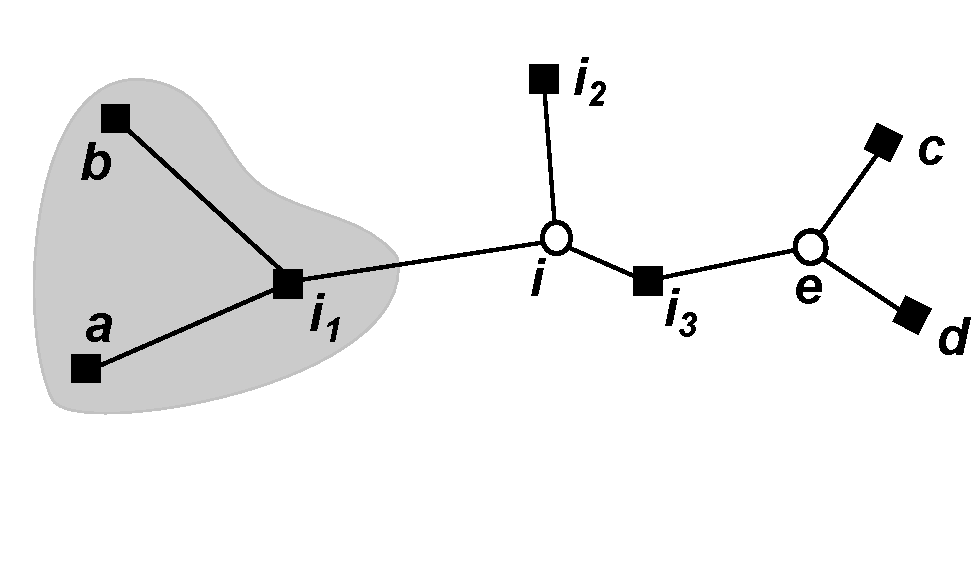
\includegraphics[height=1.6in]{objexp}
	\caption{A simple feasible solution illustrating the calculation of a contribution of node $i$ to the objective function.
		 Destinations and Steiner nodes are denoted by solid squares and empty circles, respectively.}
	\label{fig:objexp}
\end{figure}
%
The objective function captures the entire network structure, and takes account of the  frequency of usage of certain power levels.
In the example above, node $i$ uses power level $p_{ii_2}$ every time source of the relayed signal lies in the subtree $T_{i_1/i}$ which contains three potential sources.
The power level $p_{ii_1}$ is used  whenever the source lies outside of $T_{i_1/i}$, which applies to four sources.
The contribution of node $i$ to the objective function is thus $3p_{ii_2} + 4p_{ii_1}$.
The total cost of $T$ is the sum over all nodes' contributions.
In general, the total power consumption, or cost, is
$$
c(T) = \sum\limits_{i\in V_T}\left[\text{nod}(T_{i_1/i})p_{ii_2} + \text{nod}(T\setminus T_{i_1/i})p_{ii_1}\right].
$$ 
\begin{problem}
\label{def:problem}
(SMT): Find a Steiner tree $T$ of $(G,D)$ minimizing $c(T)$.
\end{problem}
Like most of the wireless network design problems presented in the literature, SMT is NP-hard. This follows from the NP-hardness of SBT\cite{Papadimitriou06SBT}, which is the special case of Problem \ref{def:problem} where $D=V$.

\section{MILP Formulations}
\label{sec:ILP}

In this section, we state and explain MILP formulations of the SMT problem.
A basic element of every MIP formulation for SMT is a set of constraints modelling a Steiner tree.
We investigate two such Steiner tree models with variables of up to 3 node indices and compare SMT models based on them.
Both models are subsequently strengthened by valid inequalities.
Variables with 4 node indices and associated constraints further extend the models.
Valid inequalities added to the extended models result in the strongest known SMT formulations.

\subsection{Formulation based on broadcast trees}

The first model extends the SBT formulation introduced in \cite{Haugland12Dual} by the Steiner nodes in order to formulate the multicast version of the problem \cite{ivanova16isco}.

\subsubsection{Underlying Steiner tree formulation [$\mathcal{X}_0$]}

Following \cite{Haugland12Dual}, define the binary variables
\newline\newline
$y_{ij}=
\begin{cases}
    1 & \text{if edge $\{i,j\} \in E$ is in the solution},\\
    0 & \text{otherwise},
  \end{cases}$
\newline\newline
$X^{s}_{ij}=
\begin{cases}
    1 & \text{if arc $(i,j) \in A$ is on a path from $s\in D$ in $G_y$},\\
    0 & \text{otherwise}.
  \end{cases}$
\newline\newline
The following constraints imply that $G_y$ is a Steiner tree spanning $D$.
The minimum Steiner tree is formulated as
%%%%%%%%%%%%%%%%%%%%%%%%%%%%%%%%%%%%%%%
%                                     % 
%     STEINER TREE MODEL $\mathcal{X}_0$           %
%                                     %
%%%%%%%%%%%%%%%%%%%%%%%%%%%%%%%%%%%%%%%
\begin{subequations}\label{mod:x0}
\begin{align}
\label{con:dd:arrowFromDest} \sum\limits_{j\in V_i}X^s_{ji} & = 1 & i,s\in D,i\neq s,\\
\label{con:dd:arrowFromNonDestB} \sum\limits_{j\in V_{i}}X^s_{ji} & \leq 1 & i\in V \setminus D, s\in D,\\
\label{con:dd:arrowFromNonDestA} X^s_{ij} & \leq \sum\limits_{k\in V_{i}\setminus \{j\}}X^s_{ki} & i\in V \setminus D,(i,j)\in A, s\in D,\\
\label{con:dd:oneDir} X^s_{ij} + X^s_{ji} & = y_{ij} & \{i,j\}\in E, s\in D,\\
\label{con:dd:startInSource} X^s_{js} & = 0 &  s\in D, (j,s)\in A,&\\
\label{con:dd:vardim}y \in \{0,1\}^{E}, X & \in \{0,1\}^{A\times D}.
\end{align}~
\end{subequations}

Let $(X,y)$ be an optimal solution to $\mathcal{X}_0$.
Then for each $s\in D$, $X^s\in \{0,1\}^{A}$ induces a Steiner arborescence $G_{X^s}$ rooted at source $s$.
From $y\in \{0,1\}^E$ we obtain the resulting (undirected) Steiner tree $G_{y}$ modeled by (\ref{con:dd:arrowFromDest})-(\ref{con:dd:startInSource}).
Constraint (\ref{con:dd:arrowFromDest}) ensures that there is exactly one predecessor $j\in V$ of a destination $i\in D$ in $G_{X^s}$.
Analogously, (\ref{con:dd:arrowFromNonDestB}) covers the case when $i \in V\setminus D$: for every source $s$, there is at most one inbound arc to a non-destination $i$.
If there is an arc $(i,j)$ in $G_{X^s}$ for a non-destination $i$, there must also be an arc $(k,i)$ such that $k\neq j$.
This is enforced by (\ref{con:dd:arrowFromNonDestA}).
Expression (\ref{con:dd:oneDir}) ensures that an edge $\{i,j\}$ is part of the resulting Steiner tree $G_{y}$ if and only if for every $s\in D$, either $(i,j)$ or $(j,i)$ is in $G_{X^s}$.
The next constraint (\ref{con:dd:startInSource}) expresses that $s$ does not have any inbound arc in $G_{X^s}$, which implies non-existence of a directed cycle containing $s$.
%Note that assuming there is no outgoing arc from a non-destination $j$, (\ref{con:dd:arrowFromNonDestA}) does not prevent $j$ from being a leaf in $G_{\mathbf{X^s}}$.
%Even though such solutions do not change the objective value of an integral solution, a Steiner tree by definition does not contain Steiner leaves.
%We therefore disallow them by adding constraint (\ref{con:dd:extraCon}) reducing the set of feasible solutions.

Conversely, for any Steiner tree $T$ spanning $D$, there exists a pair $(X,y)$ satisfying the constraints such that $G_y=T$. 

\subsubsection{SMT model [$\mathcal{X}_1$]}

A Steiner arborescence for $G_{X^s}$ can be regarded as a broadcast arborescence describing how a signal initiated in $s$ is routed towards remaining destinations. 
Then, it can also be understood that $X_{ij}^s=1$ if and only if arc $(i,j)$ is used to transmit a signal from $s\in D$.
With this notion, consider variables
\newline\newline
$\pi^s_{ij}=
\begin{cases}
    1 & \text{if $i\in V$ uses power $p_{ij}$ to transmit a message from $s\in D$ in $G_y$},\\
    0 & \text{otherwise},
  \end{cases}$
\newline\newline
leading to the following formulation $\mathcal{X}_1$ of SMT:

%%%%%%%%%%%%%%%%%%%%%%%%%%%%%%%%%%%%%%%
%                                     % 
%             MODEL $\mathcal{X}_1$                %
%           (3 idx vars)              %
%%%%%%%%%%%%%%%%%%%%%%%%%%%%%%%%%%%%%%%
\begin{subequations}[resume]\label{eq:smt-x2}
\begin{align}
\label{objective:mf} \makebox[0pt][l]{$\displaystyle{} \min \sum\limits_{(i,j) \in A} \sum\limits_{s \in D} p_{ij} \pi^s_{ij} $}\\
\notag\text{s.t.}\\
\notag(\ref{con:dd:arrowFromDest}) &- (\ref{con:dd:vardim})\\
\label{con:dd:yvar} X^s_{ij} & \leq \sum\limits_{k\in V_i:p_{ik}\geq p_{ij}}\pi^s_{ik} & s\in D, (i,j)\in A,\\
\label{con:dd:vardimy} \pi & \in \{0,1\}^{A\times D}.
\end{align}~
\end{subequations}

This model is a slightly modified version of the SMT model introduced in \cite{ivanova16isco}, which contains a constraint disallowing non-destination leaves and a weaker version of constraint (\ref{con:dd:arrowFromNonDestA}).
By (\ref{con:dd:yvar}), we define a relation between $X$-variables and $\pi$-variables used in the objective function.
Whenever the arc $(i,j)$ is used for transmission of a message from $s\in D$, the power assigned to node $i$ must be at least $p_{ij}$.
In an optimal solution $(X,y,\pi)$ to $\mathcal{X}_1$, $\pi^s\in \{0,1\}^{A}$ describes links determining the power levels used by nodes when relaying a message originated in $s$.
The graph induced by $\pi^s$ is  a subgraph of the tree induced by $X^s$, and is not necessarily connected.

\subsubsection{Valid inequalities [$\mathcal{X}_2$]}

It is possible to strengthen $\mathcal{X}_1$ by adding valid inequalities
%%%%%%%%%%%%%%%%%%%%%%%%%%%%%%%%%%%%%%%
%                                     % 
%             MODEL $\mathcal{X}_2$                %
%      (3 idx vars + VIs )            %
%%%%%%%%%%%%%%%%%%%%%%%%%%%%%%%%%%%%%%%
\begin{subequations}[resume]
\begin{align}
\label{con:dd:extraCon} \sum\limits_{j\in V_{i}}X^s_{ji} & \leq \sum\limits_{j\in V_{i}}X^s_{ij}  & 	i\in V\setminus D, s\in D,\\
\label{con:vi:Y1} \sum\limits_{j\in V_s}  \pi^{s}_{sj} & =1 & s\in D,\\
\label{con:vi:sumYImpSumX} \sum\limits_{j\in V_i\setminus\{s\} }\pi^{s}_{ij} & \geq \sum\limits_{j\in V_i}  X^{s}_{ji} & i\in V\setminus D, s\in D.
\end{align}
\end{subequations}
Constraint (\ref{con:dd:extraCon}) ensures that $G_{X^s}$, and also any feasible solution, does not contain Steiner nodes as leaves, i.e., a signal never disappears in a non-destination.
%Even though the presence of such leaves does not increase the objective value of an integral solution, it is desirable to eliminate them, because by definition, a Steiner tree does not contain non-destination leaves.
Inequality (\ref{con:vi:Y1}) says that there has to be exactly one neighbour $j\in V$ of $s\in D$, such that $s$ uses the power $p_{sj}$ in order to transmit its own signal.
As (\ref{con:vi:sumYImpSumX}) states, if a non-destination $i$ receives a signal from $s$, then there is a node $j\in V_i\setminus\{s\}$ to which the signal is forwarded requiring power $p_{ij}$ assigned to node $i$.
Index $s$ is excluded from the summation set on the left of (\ref{con:vi:sumYImpSumX}), because (\ref{con:dd:startInSource}) implies that $\pi_{is}^s=0$ is feasible, and $p_{is}\geq 0$ implies that it is optimal in $\mathcal{X}_2$. 

\subsubsection{Point to point extension [$\mathcal{X}_3$]}
\label{sec:smtx2}

This section introduces variables describing an arc on a path between two destinations, and shows how additional constraints can strengthen model $\mathcal{X}_2$.

Consider a directed path from $s\in D$ to $t\in D$.
For this purpose, let $S=\{(s,t)\in D\times D, s\neq t\}$ be the set of ordered pairs of distinct destinations.
In order to model the connectivity requirements, we introduce variables
\newline\newline
$x_{ij}^{st}=
\begin{cases}
    1 & \text{if arc $(i,j) \in A$ lies on a path from $s$ to $t$ in $G_y$, $(s,t)\in S$},\\
    0 & \text{otherwise}.
\end{cases}$
\newline\newline

Model $\mathcal{X}_2$ can be strengthened by constraints concerning the newly introduced variables, which yields model $\mathcal{X}_3$: 
\newline
\newline
%%%%%%%%%%%%%%%%%%%%%%%%%%%%%%%%%%%%%%%
%                                     % 
%             MODEL $\mathcal{X}_3$                %
%             (4 idx vars)            %
%%%%%%%%%%%%%%%%%%%%%%%%%%%%%%%%%%%%%%%
\begin{subequations}[resume]\label{eq:smt-x2}
\begin{align}
\notag\makebox[0pt][l]{$\displaystyle{} \min \sum\limits_{(i,j) \in A} \sum\limits_{s \in D} p_{ij} \pi^s_{ij} $}\\
\text{s.t.} \notag \\
(\ref{con:dd:arrowFromDest}) - (\ref{con:dd:vardim}) &\text{ and }(\ref{con:dd:yvar}) - (\ref{con:vi:sumYImpSumX}) \notag\\
\label{con:mf:flowNormal} \sum\limits_{\substack{ j\in V_i}}x^{st}_{ij}-\sum\limits_{\substack{j\in V_i }}x^{st}_{ji} & = 0 & (s,t)\in S, i\in V\setminus\{s,t\},\\
%\label{con:mf:flowDest} \sum\limits_{\substack{ j\in V_t }}x^{st}_{tj}-\sum\limits_{\substack{j\in V_t}}x^{st}_{jt}    & = -1  & (s,t)\in S,\\
\label{con:mf:flowDest} \sum\limits_{\substack{j\in V_t}}x^{st}_{jt}    & = 1  & (s,t)\in S,\\
\label{con:mf:fcap} x^{st}_{ij} &\leq X^{s}_{ij}& (i,j)\in A, (s,t)\in S,\\
\label{con:mf:fsym} x^{st}_{ij} &=  x^{ts}_{ji}& (i,j)\in A, (s,t)\in S,\\ 
%\label{con:vi:f2dest}  x^{st_1}_{ij}-x^{st_2}_{ij}+x^{t_1t_2}_{ij} & \geq 0 & (i,j) \in A,\\
%\notag && (s,t_1),(s,t_2),(t_1,t_2)\in S,\\
%\label{con:vi:xImpSumF} X^{s}_{ij} & \leq \sum\limits_{t\in D_s}  x^{st}_{ij} & (i,j)\in A, s\in D, \\
\label{con:vi:sumFImpSumY} \sum\limits_{k\in V_j, p_{jk}\geq p_{ji}}x^{st}_{jk} & \leq \sum\limits_{k\in V_j, p_{jk}\geq p_{ji}}  \pi^{s}_{jk} & i,j\in V, (s,t)\in S,\\
\label{con:mf:xydim} x&\in\{0,1\}^{A\times S}. 
\end{align}~
\end{subequations}

The flow conservation constraints (\ref{con:mf:flowNormal})-(\ref{con:mf:flowDest}) guarantee that for each $(s,t)\in S$, there exists a directed path from $s$ to $t$.
Next, constraint (\ref{con:mf:fcap}) expresses the obvious relation between $X$ and $x$, that if an arc $(i,j)$ lies on a path from $s$ to $t$, then this arc is also on a path from $s$.
The flow symmetry (\ref{con:mf:fsym}) states that arc $(i,j)$ lies on a path from $s$ to $t$ if and only if arc $(j,i)$ lies on a path from $t$ to $s$.

In terms of broadcast trees, we can say that $x_{ij}^{st}=1$ if and only if $(i,j)$ carries a signal initiated in $s$ and directed to $t$.
Consider nodes $i,j\in V$ and a pair of destinations $(s,t)$.
If a message from $s$ to $t$ is sent through $(j,k)$ such that $p_{jk}\geq p_{ji}$, then the message from $s$ must be relayed by $j$ using power level at least $p_{ji}$.
This is expressed by valid inequality (\ref{con:vi:sumFImpSumY}).

\subsection{Formulation based on network flows}

There are many formulations for the Steiner minimum tree problem that can serve as a basis for modelling SMT.
We consider the multi-commodity network flow based model studied in \cite{Polzin}, where the authors use abbreviation $P_{F}$.
The model assumes a given destination $s_0\in D$ that plays the role of a unique source.
To simplify the notation, let $D_0= D_{s_0}$.

\subsubsection{Underlying Steiner tree formulation [$\mathcal{F}_0$]}

The model $\mathcal{F}_0$ of a Steiner tree contains variables
%
\newline\newline
  $g_{ij}=
\begin{cases}
    1 & \text{if arc $(i,j) \in A$ is a part of the solution},\\
    0 & \text{otherwise},
\end{cases}$
\newline\newline
  $F^{t}_{ij}=
\begin{cases}
    1 & \text{if arc $(i,j) \in A$ lies on a path from $s_0$ to $t\in D_0$ in $G_g$},\\
    0 & \text{otherwise},
\end{cases}$
\newline\newline
%
and is formulated as
%%%%%%%%%%%%%%%%%%%%%%%%%%%%%%%%%%%%%%%
%                                     % 
%     STEINER ARBORESCENCE $\mathcal{F}_0$         %
%        (from Polzin)                %
%%%%%%%%%%%%%%%%%%%%%%%%%%%%%%%%%%%%%%%
\begin{subequations}
\begin{align}
%\makebox[0pt][l]{$\displaystyle{}\min \sum\limits_{(i,j) \in A} p_{ij} g_{ij} $}  \\ \notag
%\text{s.t.} && \\
\label{con:pf1:xfrel} F^{t}_{ij} & \leq g_{ij} & t\in D_0, (i,j)\in A, \\
\label{con:pf1:flow} \sum\limits_{\substack{ j \in V_i }}F^{t}_{ji}-\sum\limits_{\substack{j\in V_i}}F^{t}_{ij} &= 
  \begin{cases}
    1 & t\in D_0, t = i,\\
    0 & t\in D_0, i\in V\setminus \{s_0, t\},
  \end{cases}\\
%\label{con:pf1:yvar} g_{ij} - F^t_{ij}+F^t_{ji} & \leq \sum\limits_{\substack{k\in V: \\ p_{ik}\geq p_{ij}}}\pi^t_{ik}  & t\in D_0, (i,j)\in A,\\
%\label{con:pf1:yvar0} g_{ij} & \leq \sum\limits_{\substack{k\in V: \\ p_{ik}\geq p_{ij}}}\pi^0_{ik}   &  (i,j)\in A,\\
%\label{con:pf1:B}  \sum_{j\in V_i}g_{ji}&\leq 1 & i\in V\setminus D,\\
%\label{con:pf1:noflowFromT} F_{ti}^t&=0 & t\in D_0, i\in V_t,\\
%\label{con:pf1:fitt=xit} F_{it}^t&=g_{it} & t\in D_0, i\in V_t,\\
%\label{con:pf1:xi0=0} g_{i0}&=0 & i\in V_0,\\
\label{con:pf1:dim}g \in \{0,1\}^{A},F&\in\{0,1\}^{A \times D_0}.
%\label{con:pf1:dimy} y&\in \{0,1\}^{A\times D}.
\end{align}~
\end{subequations}

The $g$-variables inducing the resulting tree correspond to arcs, whereas analogous $y$-variables in $\mathcal{X}_0$ correspond to edges.
Hence, an optimal solution to $\mathcal{X}_0$ is an undirected tree, and an optimal solution to $\mathcal{F}_0$ is an arborescence rooted at $s_0$.
The vector $F^t$ defines a directed path from $s_0$ to $t\in D$ in the arborescence.
Constraints (\ref{con:pf1:xfrel})-(\ref{con:pf1:flow}) together with (\ref{con:pf1:dim}) imply that $g$ induces an arborescence spanning $D$ with node $s_0$ as the root.

We aim to create an SMT model $\mathcal{F}_1$ based on $\mathcal{F}_0$.
For this purpose, it is necessary to find a way to represent the constraint (\ref{con:dd:yvar}) in the $\mathcal{F}_1$ space.
The $\pi$-variables from $\mathcal{X}_1$ have to be used in $\mathcal{F}_1$, because they appear in the objective function which remains unchanged.

\subsubsection{SMT model [$\mathcal{F}_1$]}

The model $\mathcal{F}_1$ for Problem \ref{def:problem} based on the minimum Steiner arborescence model $\mathcal{F}_0$ is constructed as follows: 
%%%%%%%%%%%%%%%%%%%%%%%%%%%%%%%%%%%%%%%
%                                     % 
%             MODEL $\mathcal{F}_1$                %
%        (3 idx vars)                 %
%%%%%%%%%%%%%%%%%%%%%%%%%%%%%%%%%%%%%%%
\begin{subequations}[resume]
\begin{align}
\notag\min & \sum\limits_{(i,j) \in A} \sum\limits_{s \in D} p_{ij} \pi^s_{ij}\\ 
\notag\text{s.t.} && \\
\notag(\ref{con:pf1:xfrel}) - (\ref{con:pf1:dim})\\
\label{con:pf1:yvar} g_{ij} - F^t_{ij}+F^t_{ji} & \leq \sum\limits_{\substack{k\in V: \\ p_{ik}\geq p_{ij}}}\pi^t_{ik}  & t\in D_0, (i,j)\in A,\\
\label{con:pf1:yvar0} g_{ij} & \leq \sum\limits_{\substack{k\in V: \\ p_{ik}\geq p_{ij}}}\pi^0_{ik}   &  (i,j)\in A,\\
\label{con:pf1:B}  \sum_{j\in V_i}g_{ji}&\leq 1 & i\in V\setminus D,\\
\label{con:pf1:noflowFromT} F_{ti}^t&=0 & t\in D_0, i\in V_t,\\
\label{con:pf1:fitt=xit} F_{it}^t&=g_{it} & t\in D_0, i\in V_t,\\
\label{con:pf1:xi0=0} g_{i0}&=0 & i\in V_0,\\
\label{con:pf1:dimy} \pi&\in \{0,1\}^{A\times D}.
\end{align}~
\end{subequations}

Constraints (\ref{con:pf1:yvar}) and (\ref{con:pf1:yvar0}) have the same purpose as (\ref{con:dd:yvar}), and are expressed in $\mathcal{F}_1$ space. % using transformations (\ref{eq:tr:xijsB}).
Note that the $\pi$-variables determining power levels are defined for all destinations in $D$, while in the model $\mathcal{F}_1$ \cite{Polzin} of the minimum Steiner tree problem, the $F$-variables are defined only for destinations in $D_0$.
For this reason, $\pi_{ij}^0$ is treated separately in (\ref{con:pf1:yvar0}).
%This inconsistency is resolved by adding (\ref{con:pf1:yvar0}), which relates the $\pi^0$-variables with $x$-variables. This is equivalent to extending the the domain of the $f$-variables and fixing the newly introduced variables to zero. 

By (\ref{con:pf1:B}) we prevent a non-destination from having multiple entering arcs.
This is not needed in the minimum Steiner tree problem formulation, because the objective function causes that such solutions are filtered out by optimality.
The necessity of this constraint in SMT is demonstrated in Fig. \ref{fig:BProof}.
%The optimal solution with objective value 25156 to the depicted instance obtained by solving SMT-$\mathcal{X}_1$ is shown in Fig. \ref{fig:BorigSMT}.
%The solution in Fig \ref{fig:Bpf2} yielded by solving SMT-$\mathcal{F}_1$ without the constraint (\ref{con:pf1:B}) has objective value 25148, but is not a feasible solution to Problem \ref{def:problem}, because of the cycle $(g,h,i,d,g)$.
%The non-existence of such a cycle in a solution given by model $\mathcal{X}_1$ is ensured by constraints (\ref{con:dd:arrowFromDest}), (\ref{con:dd:arrowFromNonDestB}) and (\ref{con:dd:oneDir}).
%A detailed proof of this claim can be found in \cite{ivanova16isco}.
%A transmission commenced in node $c$ is sent via arc $(g,f)$.
%As a consequence of the link between $g$ and $d$ in Fig. \ref{fig:Bpf2}, the node $d$ also receives the message.
%This link is absent in Fig. \ref{fig:BorigSMT}, and so $i$ has to relay the signal using arc $(i,d)$, causing the higher total objective value.
Similarly, the obviously valid inequalities (\ref{con:pf1:noflowFromT})-(\ref{con:pf1:fitt=xit}) are not necessary in the minimum Steiner tree formulation, but have to be included in the formulation of SMT, because they  disallow nodes in $D_0$ to have multiple entering arcs.
The same restriction has to be imposed on $s_0$ by including (\ref{con:pf1:xi0=0}).
%%%%%%%%%%%%%%%%%%%%%%%%%%%%%%%%%%%%%%%%%%%%%%%%%%%%%%
%      Figure                                        %
%    explaining why some constraints are necessary   %
%%%%%%%%%%%%%%%%%%%%%%%%%%%%%%%%%%%%%%%%%%%%%%%%%%%%%%
\begin{figure}[!htb]
    \centering
    \begin{subfigure}[b]{0.4\textwidth}
        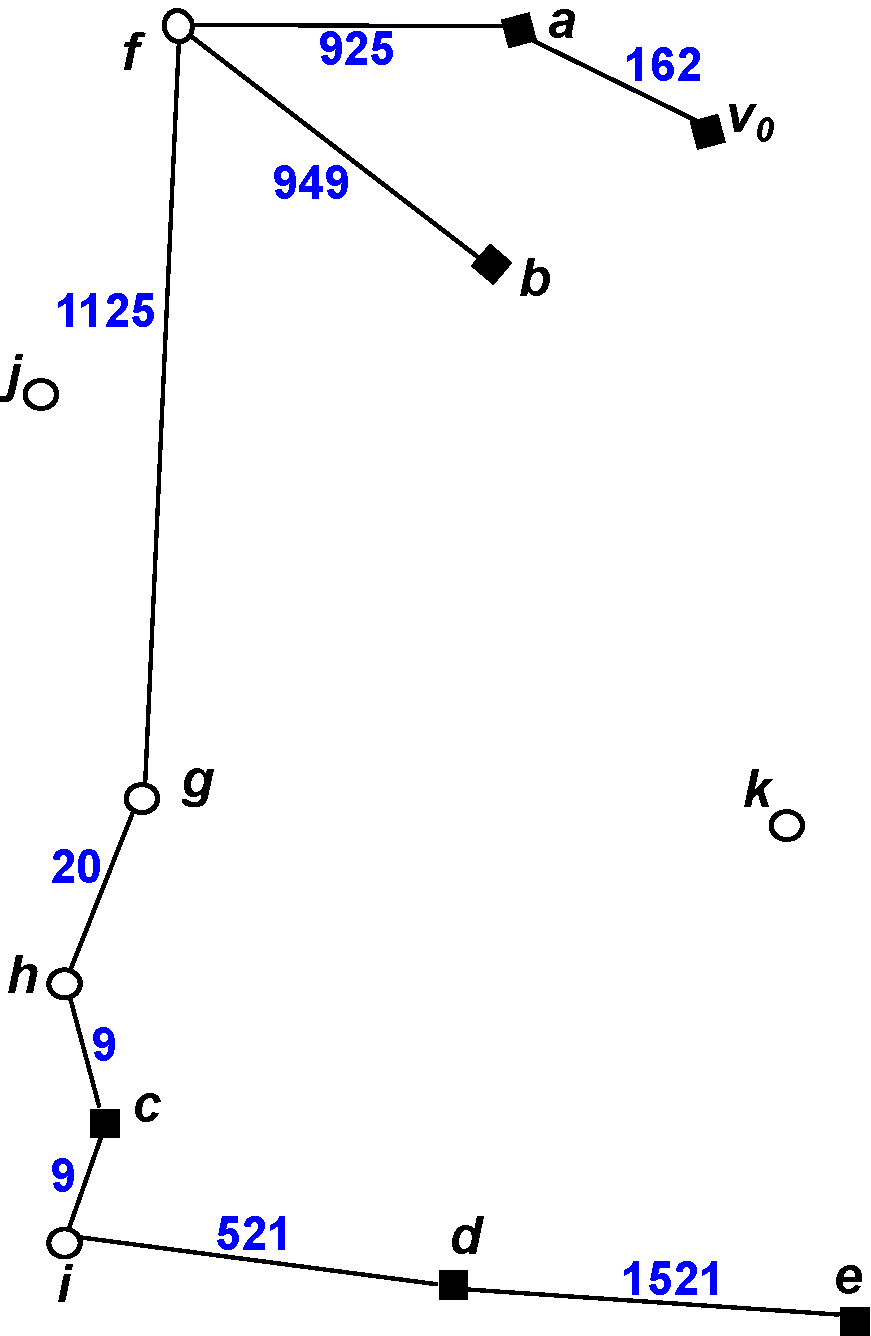
\includegraphics[width=\textwidth]{conBNec}
        \caption{Optimal solution obtained by $\mathcal{X}_1$. The $y$-variables inducing the resulting tree in this model represent undirected edges. The objective value of this tree is 25156.\newline~}
        \label{fig:BorigSMT}
    \end{subfigure}
    \hfill
% a blank line to force the subfigure onto a new line
    \begin{subfigure}[b]{0.4\textwidth}
        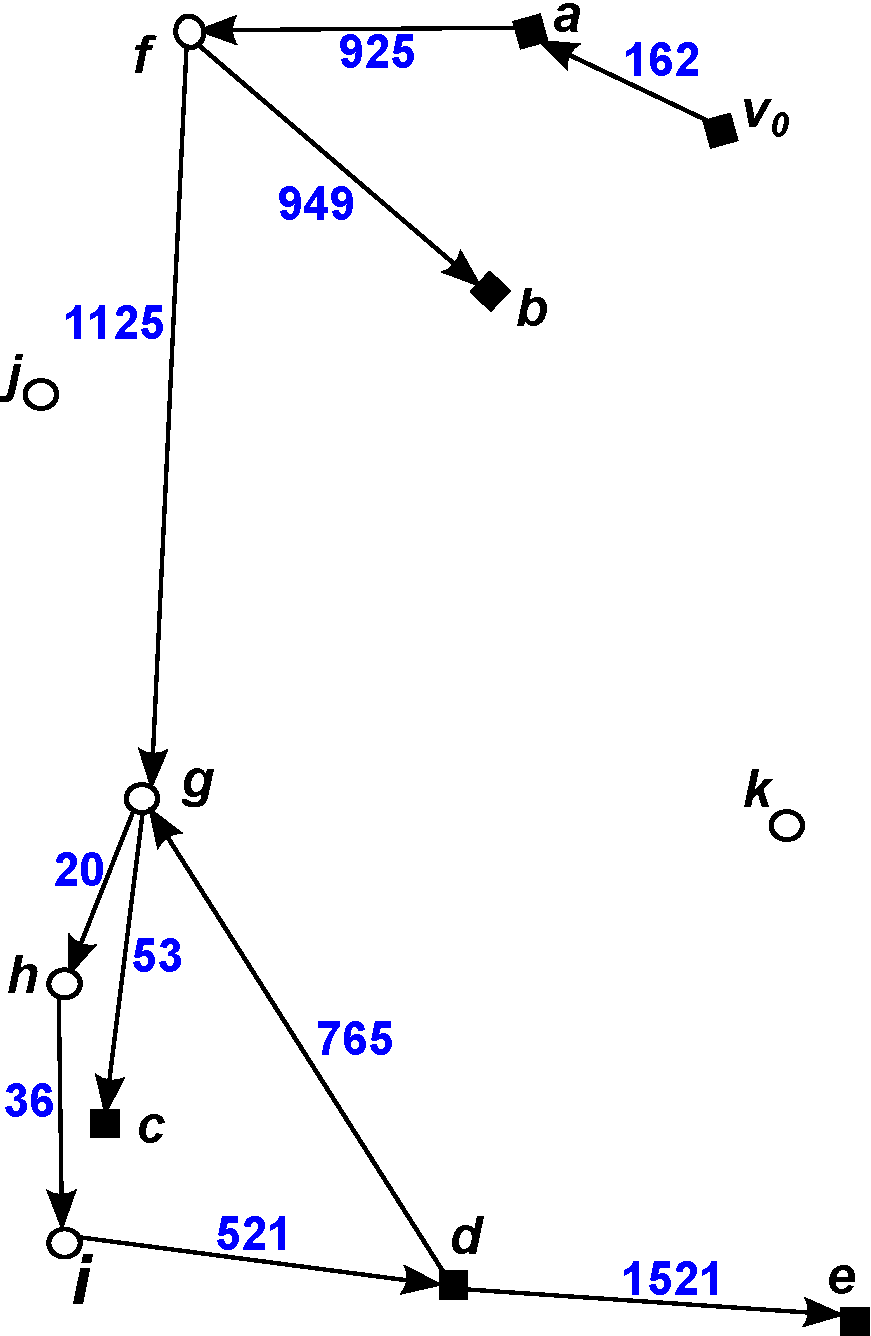
\includegraphics[width=\textwidth]{conBNec2}
        \caption{Solution obtained by $\mathcal{F}_1$ without constraint \ref{con:pf1:B} with objective value 25148 is not a Steiner tree.
		 The nodes are connected by arrows because the solution is a directed graph with a predefined source $s_0$.}
        \label{fig:Bpf2}
    \end{subfigure}
    \caption{An exemplary instance showing why constraint (\ref{con:pf1:B}) is necessary in $\mathcal{F}_1$.
		Blue numbers denote power requirements of connection between nodes.
		For better legibility, the distances of the links are not proportional.} 
    \label{fig:BProof}
\end{figure}

%%%%%%%%%%%%%%%%%%%%%%%%%%%%%%%%%%%%%%%
%                                     %
%         Proposition  		      %
% ($\mathcal{F}_1$ models an arborescence) %
%                                     %
%%%%%%%%%%%%%%%%%%%%%%%%%%%%%%%%%%%%%%%
\begin{prop}
\label{prop:modelcorrect}
If $(F,g)$ satisfies (\ref{con:pf1:xfrel}) - (\ref{con:pf1:dim}) and (\ref{con:pf1:B})-(\ref{con:pf1:xi0=0}) then $G_{g}$ is a Steiner arborescence spanning $D$ rooted at $s_0$.
\end{prop}
 
\begin{proof}
The connectivity of $G_{g}$ as well as coverage of all nodes from $D$ is ensured by flow constraints (\ref{con:pf1:flow}) and relation (\ref{con:pf1:xfrel}).
The absence of both directed and undirected cycles is enforced by (\ref{con:pf1:B})-(\ref{con:pf1:xi0=0}).
As discussed above, these constraints together imply that no node has more than one entering arc.
In particular for a destination $i\in D_0$, by utilizing first (\ref{con:pf1:fitt=xit}), next (\ref{con:pf1:flow}) for $t=i$, and finally (\ref{con:pf1:noflowFromT}), we get
$$\sum_{j\in V_i}g_{ji}=\sum_{j\in V_i}F_{ji}^i = 1+\sum_{j\in V_i}F_{ij}^i=1.$$
%Solutions, where nodes from $V\setminus D$ are leaves are excluded due to (\ref{con:pf1:flowX}).
\qed
\end{proof}


%%%%%%%%%%%%%%%%%%%%%%%%%%%%%%%%%%%%%%%
%                                     %
%         Proposition  		      %
%   (transformation X_{ij}^s)         %
%                                     %
%%%%%%%%%%%%%%%%%%%%%%%%%%%%%%%%%%%%%%%
\begin{prop}\label{prop:transX}
Assume $(F,\pi,g)$ satisfies (\ref{con:pf1:xfrel}) - (\ref{con:pf1:dim}) and  (\ref{con:pf1:B}) - (\ref{con:pf1:dimy}). Then
$$
g_{ij} - F^t_{ij}+F^t_{ji} = 
	\begin{cases}
		1, ~(i,j)~\text{is an arc on the path from~$t\in D_0$ in $G_{g}$} \\
		0, ~\text{otherwise.}
	\end{cases}
$$
\end{prop}
%
\begin{proof}
Let $T=(V_T,E_T)$ be a tree covering $D$ induced by $g$, and consider an edge $\{i,j\}\in E_T$ dividing $T$ into two subtrees $T_i$ and $T_j$ rooted in $i$ and $j$, respectively.
Assume without loss of generality that $t\in T_i$.
Either $s_0$ and $t$ are both in $T_i$, in which case none of the arcs $(i,j)$ and $(j,i)$ carries a flow to $t$, or $s_0$ belongs to $T_j$, and there is a flow from $s_0$ via $(j,i)$ towards $t$.
That is expressed in F-space as
$
g_{ij}(1-F^{t}_{ij})(1-F^{t}_{ji})+g_{ji}F^{t}_{ji}=g_{ij} - F^t_{ij}+F^t_{ji},
$
where the equality follows from (\ref{con:pf1:xfrel}).
\qed
\end{proof}

\begin{cor}
$\mathcal{F}_1$ is a correct formulation of Problem \ref{def:problem}.
\end{cor}

\subsubsection{Valid inequalities [$\mathcal{F}_2$]}

The same valid inequalities  leading to $\mathcal{X}_2$ are added to $\mathcal{F}_1$, resulting in the model denoted as $\mathcal{F}_2$.
Inequality (\ref{con:vi:Y1}) is added without any change.
The $x$-variable in (\ref{con:vi:sumYImpSumX}) has to be replaced by the equivalent expression from Prop. \ref{prop:transX}. 
Subsequent application of flow conservation (\ref{con:pf1:flow}) yields
%%%%%%%%%%%%%%%%%%%%%%%%%%%%%%%%%%%%%%%
%                                     %
%             MODEL $\mathcal{F}_2$                %
%                                     %
%%%%%%%%%%%%%%%%%%%%%%%%%%%%%%%%%%%%%%%
\begin{subequations}[resume]
\begin{flalign}
\label{con:vi:sumYImpSumXTrans} \sum\limits_{j\in V_i }\pi^{s}_{ij} & \geq \sum\limits_{j\in V_i}  g_{ji}  \quad\quad   i\in V\setminus D, s\in D. 
\end{flalign}
\end{subequations}
%
Further strengthening can be achieved by including 
\begin{subequations}[resume]
\begin{flalign}
\label{con:pf1:flowX}  \sum\limits_{\substack{ j\in V_i }}g_{ji}-\sum\limits_{\substack{j\in V_i}}g_{ij}    & \leq 0    \qquad\qquad			  i\in V\setminus D 
\end{flalign}
\end{subequations}
introduced in \cite{Polzin}, which is also analogous to (\ref{con:dd:extraCon}).
%This constraint is analogous to ($\ref{con:dd:extraCon})$, and is also obtained by applying (\ref{eq:tr:xijsB}) together with (\ref{con:pf1:flow}).

\subsubsection{Double flow extension [$\mathcal{F}_3$]}

Similarly to the extension $\mathcal{X}_3$ of $\mathcal{X}_2$ by $x$-variables, the model $\mathcal{F}_2$ can also be extended by variables with four node indices.
Analogously to $S$, let $\check{S}=\{\{s,t\}\subseteq D: s\neq t\}$ be the set of unordered pairs of destinations, and let $\check{S}_0=\{\{s,t\}\in S: s\neq s_0\neq t\}$.
 
The authors of \cite{Polzin} use variables
\newline\newline
$f^{st}_{ij}=
\begin{cases}
    1 & \text{if arc $(i,j) \in A$ lies on an intersection of  paths from $s_0$ } \\
    ~ & \text{to $s$ and $t$ in $G_g$, $\{s,t\}\in \check{S}_0$},\\
    0 & \text{otherwise},
\end{cases}$
\newline\newline
which can also be regarded as a description of a common flow from $s_0$ to $s$ and $t$.
%describing a common flow from $s_0$ to $s$ and $t$.
%It is now possible to express variables $x^{st}_{ij}$ from $$\mathcal{X}_2$$ in the $\mathcal{F}_3$ space as 
%
%\begin{align}
%\label{eq:tr:fstij1}
%\begin{aligned}
%x^{st}_{ij}&=F^t_{ij}(1-f^{st}_{ij})+F^{s}_{ji}(1-f^{st}_{ji})= \\
%  	   &=  F^t_{ij}+F^s_{ji} - f^{st}_{ij} - f^{st}_{ji}\\
%x^{0t}_{ij}&=F^t_{ij}\\
%\end{aligned}
%&&
%\begin{aligned}
%\\
%(i,j)\in A, \{s,t\}\in S_0\\
%(i,j)\in A, t\in S_0.
%\end{aligned}
%\end{align}
%
This allows formulation of an extended model denoted as $\mathcal{F}_3$: 
%%%%%%%%%%%%%%%%%%%%%%%%%%%%%%%%%%%%%%%
%                                     %
%             MODEL $\mathcal{F}_3$   %
%                                     %
%%%%%%%%%%%%%%%%%%%%%%%%%%%%%%%%%%%%%%%
\begin{subequations}[resume]
\begin{align}
\notag\min & \sum\limits_{(i,j) \in A} \sum\limits_{s \in D} p_{ij} \pi^s_{ij}\\ \notag
\text{s.t.}& && \\
%(\ref{con:pf1:xfrel}) - (\ref{con:pf1:flowX}),& \notag \\
\notag(\ref{con:pf1:flow}) &- (\ref{con:pf1:flowX})\\
\label{con:pf2:flowHook} \sum\limits_{\substack{ j \in V_i }}f^{st}_{ji}-\sum\limits_{\substack{j\in V_i}}f^{st}_{ij} & \geq 
  \begin{cases}
    -1 & \{s,t\}\in \check{S_0}, i = 0, \\
    0  & \{s,t\}\in \check{S_0}, i\in V\setminus \{s_0\},
  \end{cases}  \\
\label{con:pf2:startInSource}  f^{st}_{ij} & \leq F^s_{ij} \quad \{s,t\}\in \check{S_0}, (i,j)\in A,\\
\label{con:pf2:stopInDest}  f^{st}_{ij} & \leq F^t_{ij} \quad \{s,t\}\in \check{S_0}, (i,j)\in A,\\
\label{con:pf2:stronger}  F^{s}_{ij}+F^{t}_{ij}-f^{st}_{ij} &\leq g_{ij} \quad \{s,t\}\in \check{S_0}, (i,j)\in A,\\ 
\label{con:pf2:sumFImpSumY} \sum\limits_{k\in V_j, p_{jk}\geq p_{ji}}F^{t}_{jk} + F^{s}_{kj} - f^{st}_{jk} - f^{st}_{kj} & \leq \sum\limits_{k\in V_j, p_{jk}\geq p_{ji}}  \pi^{s}_{jk} \quad i,j\in V,\{s,t\}\in \check{S_0},\\
\label{con:pf2:sumFImpSumY2} \sum\limits_{k\in V_j, p_{jk}\geq p_{ji}}F^{t}_{jk} & \leq \sum\limits_{k\in V_j, p_{jk}\geq p_{ji}}  \pi^{0}_{jk} \quad i,j\in V, t\in D_0,\\
\label{con:pf2:dim} f&\in\{0,1\}^{A\times \check{S}}.
\end{align}~
\end{subequations}

By (\ref{con:pf2:flowHook}) is ensured that the common flow is non-increasing.
The inequalities (\ref{con:pf2:stronger}) replace a weaker (\ref{con:pf1:xfrel}).
Finally, (\ref{con:pf2:sumFImpSumY}) - (\ref{con:pf2:sumFImpSumY2}) is a valid inequality (\ref{con:vi:sumFImpSumY}) implied by the following
%%%%%%%%%%%%%%%%%%%%%%%%%%%%%%%%%%%%%%%
%                                     %
%         Proposition  		      %
%   (transformation x_{ij}^{st})      %
%                                     %
%%%%%%%%%%%%%%%%%%%%%%%%%%%%%%%%%%%%%%%
\begin{prop}\label{prop:transX}
Assume $(F,f,\pi,g)$ satisfies (\ref{con:pf1:flow}) - (\ref{con:pf2:stronger}). Then
$$
F^t_{ij}+F^s_{ji}-f^{st}_{ij}-f^{st}_{ji} = 
	\begin{cases}
		1, ~(i,j)~\text{is an arc on the path from~$s$ to $t$ in $G_{g}$} \\
		0, ~\text{otherwise.}
	\end{cases}
$$
\end{prop}
%
\begin{proof}

Let $T=(V_T,E_T)$ be a tree covering $D$, and consider an edge $\{i,j\}\in E_T$ dividing $T$ into two subtrees $T_i$ and $T_j$ rooted in $i$ and $j$, respectively.
If the arc $(i,j)$ carries flow from $s\in D$ to $t\in D$, then $s$ and $t$ must lie in different subtrees.
Node $s_0$ lies either in $T_i$ or $T_j$.
%as depicted in Fig. \ref{fig:transf_a} and Fig. \ref{fig:transf_b}, respectively.
%These two cases are captured by the first equality in (\ref{eq:tr:fstij}).
If both $s_0$ and $s$ lie in $T_i$, then $F_{ij}^t=1$.
Similarly, if $s_0$ and $t$ lie in $T_j$, then $F_{ji}^s=1$.
We can write this as
$$
F^t_{ij}(1-f^{st}_{ij})+F^{s}_{ji}(1-f^{st}_{ji})= F^t_{ij}+F^s_{ji} - f^{st}_{ij} - f^{st}_{ji}.
$$
The expressions in parentheses prevent $s$ and $t$ belonging to the same subtree.
By relations $f^{st}_{ij}\leq F_{ij}^t=1$ and $f^{st}_{ji}\leq F_{ji}^s=1$ we obtain the desired linear expression on the right-hand side. 
\qed
\end{proof}
%%%%%%%%%%%%%%%%%%%%%%%%%%%%%%%%%%%%%%%%%%%%%%%%%%%%%%%%%%%
%	Additional VI following from implicit symmetry 5  %
%%%%%%%%%%%%%%%%%%%%%%%%%%%%%%%%%%%%%%%%%%%%%%%%%%%%%%%%%%%
%It follows from the domain of $f$, that 
%\begin{equation}
%\label{eq:fhooksym}f_{ij}^{st}=f_{ij}^{ts},
%\end{equation}
%because $S_0$ consists of unordered pairs. 
%By the implicit assumption of (\ref{eq:fhooksym}) in SMT-$\mathcal{F}_2$, it is possible to infer additional valid inequalities for SMT. We can also write
%\begin{align*}
%f^{st}_{ij}+f^{st}_{ji}=f^{ts}_{ij}+f^{ts}_{ji} &\Rightarrow F^t_{ij}+F^s_{ji}-x^{st}_{ij}=F^s_{ij}+F^t_{ji}-x^{ts}_{ij}\Rightarrow \\ & \Rightarrow x^{0t}_{ij}+x^{0s}_{ji}-x^{st}_{ij}=x^{0s}_{ij}+x^{0t}_{ji}-x^{ts}_{ij}.
%\end{align*}
%The first and second implication follow from the transformation (\ref{eq:tr:fstij}) and (\ref{eq:tr:fijt2}), respectively. The last equality consists of only variables from SMT-$\mathcal{X}_2$  space, and so the valid inequality
%\begin{equation*}
%x^{ut}_{ij}+x^{us}_{ji}+x^{ts}_{ij}=x^{us}_{ij}+x^{ut}_{ji}+x^{st}_{ij} \quad\quad (u,t),(u,s),(s,t),(t,s)\in S_0, i,j\in V
%\end{equation*}
%can be added to  SMT-$\mathcal{X}_2$. All the occurances of $s_0$ were replaced by a general destination $u\in D$, because $s_0$ does not have any special role in SMT-$\mathcal{X}_2$.

%\subsubsection{Valid inequalities [$\mathcal{F}_2$VI]}

%To complete the listing of models, we state the model $\mathcal{F}_2$VI created by adding transformed valid inequalities (\ref{con:vi:f2dest})-(\ref{con:vi:sumFImpSumY}) to $\mathcal{F}_2$.



\section{Relations Between the Models}
\label{sec:comp}

In order to create the $\mathcal{F}_1$ model, it is necessary to express variables  $X^s_{ij}$ in $\mathcal{F}_1$ space using relation (\ref{eq:tr:xijj}).
The aim of this section is to show how the entire $\mathcal{X}_2$ model can be converted into an equivalent model that uses only variables of $\mathcal{F}_2$.
 

The following equations express all variables from $\mathcal{X}_2$ in $\mathcal{F}_2$ space:
%%%%%%%%%%%%%%%%%%%%%%%%%%%%%%%%%%%%%%%
%                                     % 
%       Transformation (7)            %
%                                     %
%%%%%%%%%%%%%%%%%%%%%%%%%%%%%%%%%%%%%%%
\begin{subequations}
\begin{align}
\notag\label{eq:tr:fstij}x^{st}_{ij}&=F^t_{ij}(1- f^{st}_{ij})+F^s_{ji}(1- f^{st}_{ji})= \\
  &=  F^t_{ij}+F^s_{ji} -  f^{st}_{ij} -  f^{st}_{ji}& (i,j)\in A, \{s,t\}\in S_0\\
\notag\label{eq:tr:xijj}X^s_{ij}&=g_{ij}(1-F^s_{ij})(1-F^s_{ji})+g_{ji}F^s_{ji}=\\
  &= g_{ij}-F^s_{ij} + F^s_{ji} & (i,j)\in A, s\in D_0\\
\label{eq:tr:zij}y_{ij}&=g_{ij}+g_{ji}& \{i,j\}\in E
\end{align}
\end{subequations}
The transformations can be explained as follows:
Let $T=(V_T,E_T)$ be a tree covering $D$, and consider an edge $\{i,j\}\in E_T$ dividing $T$ into two subtrees $T_i$ and $T_j$ rooted in $i$ and $j$, respectively.
If the arc $(i,j)$ carries flow from $s\in D$ to $t\in D$, then $s$ and $t$ must lie in different subtrees.
Node $s_0$ lies either in $T_i$ or $T_j$.
%as depicted in Fig. \ref{fig:transf_a} and Fig. \ref{fig:transf_b}, respectively.
These two cases are captured by the first equality in (\ref{eq:tr:fstij}).
If both $s_0$ and $s$ lie in $T_i$, then $F^t_{ij}=1$.
Similarly, if $s_0$ and $t$ lie in $T_j$, then $F_{ji}^s=1$.
The expressions in parentheses prevent $s$ and $t$ belonging to the same subtree.
Using the implications $f^{st}_{ij}=1\Rightarrow F^t_{ij}=1$ and $f^{st}_{ji}=1\Rightarrow F_{ji}^s=1$ that follow from the interpretation of variables, we justify the second equality expressing this relation linearly.
In the transformation (\ref{eq:tr:xijj}) of $g_{ij}^s$, we distinguish the situation when $s_0$ and $s$ are in the same subtree, in which case none of the arcs $(i,j)$ and $(j,i)$ carries a flow to $s$, and when $s$ and $s_0$ belong to different subtrees, and there is a flow via $(j,i)$ towards $s$.
Again, the last equality is justified since $F_{ij}^s=1\Rightarrow g_{ij}=1$.
The relation (\ref{eq:tr:zij}) is obvious.

By a similar approach, we achieve the transformation from $\mathcal{X}_2$ space to $\mathcal{F}_2$ space. 
%%%%%%%%%%%%%%%%%%%%%%%%%%%%%%%%%%%%%%%
%                                     %
%       Transformation (8)            %
%                                     %
%%%%%%%%%%%%%%%%%%%%%%%%%%%%%%%%%%%%%%%
\begin{subequations}
\begin{align}
\label{eq:tr:xij=xij0}g_{ij}=&x^0_{ij} & (i,j)\in A\\
\label{eq:tr:fijt2}F^t_{ij}=&x^t_{ji}x^0_{ij}=f^{0t}_{ij} & (i,j)\in A, t\in D_0\\
\label{eq:tr:fstij2} f^{st}_{ij}=& x^s_{ji}x^t_{ji}x^0_{ij} & (i,j)\in A, \{s,t\}\in \check{S}_0
\end{align}
\end{subequations}

We aim to compare the models presented in Section \ref{sec:ILP} in terms of strength.
The results obtained by numerical experiments presented in the next section suggest that $\mathcal{F}_2$ model is at least as strong as $\mathcal{X}_2$.
This section proves this conjecture.
 
First, we express the $\mathcal{X}_2$ model in $\mathcal{F}_2$ space using transformations (\ref{eq:tr:fstij})-(\ref{eq:tr:zij}). 
%%%%%%%%%%%%%%%%%%%%%%%%%%%%%%%%%%%%%%%
%                                     %
%             MODEL (9)               %
%                                     %
%%%%%%%%%%%%%%%%%%%%%%%%%%%%%%%%%%%%%%%
\begin{subequations}
\begin{flalign}
\label{objective:mfinpf2} &\makebox[0pt][l]{$\displaystyle{}\min \sum\limits_{(i,j) \in A} \sum\limits_{s \in D} p_{ij} \pi^s_{ij} $} & \\ 
\notag\text{s.t.}& & \\
\label{con:mfinpf2:arrowFromDest} \sum\limits_{j\in V_i}(g_{ji}-F^s_{ji}+F^s_{ij}) & = 1 & i\in D, s\in D, i \neq s,\\ 
\label{con:mfinpf2:arrowFromNonDestB} \sum\limits_{j \in V_i}(g_{ji}-F^s_{ji}+F^s_{ij}) &\leq 1 & i\in V \setminus D, s\in D,\\
\label{con:mfinpf2:arrowFromNonDestA} g_{ij}-F^s_{ij}+F^s_{ji}  & \leq \sum\limits_{k \in V_i\setminus\{j\}}(g_{ki}-F^s_{ki}+F^s_{ik}) & i\in V \setminus D,\\
\notag & & j\in V_i, s\in D,\\
\label{con:mfinpf2:startInSource} x_{js} - F^s_{js}+F^s_{sj} & = 0 & s\in D, j\in V_s,\\
\label{con:mfinpf2:yvar} g_{ij}-F^s_{ij}+F^s_{ji} & \leq \sum\limits_{k\in V:p_{ik}\geq p_{ij}}\pi^s_{ik} & s\in D, (i,j)\in A,\\ 
\label{con:mfinpf2:extraCon} \sum\limits_{j\in V_{i}}\left(g_{ji}-F^s_{ji}+F^s_{ij}\right) & \leq \sum\limits_{j\in V_{i}}\left(g_{ij}-F^s_{ji}+F^s_{ij}\right)  &\in V\setminus D, s\in D,\\
\notag\text(\ref{con:vi:Y1}) & &\\
\label{con:mfinpf2:sumYImpSumXTrans} \sum\limits_{j\in V_i\setminus\{s\} }\pi^{s}_{ij} & \geq \sum\limits_{j\in V_i} \left( g_{ji}-F^s_{ji}+F^s_{ij} \right) &  i\in V\setminus D, s\in D,\\ 
\label{con:mfinpf2:flowNormal}  \sum\limits_{\substack{ j\in V_i }}(F^t_{ij}+F^s_{ji})&=\sum\limits_{\substack{j\in V_i }}(F^t_{ji}+F^s_{ij}) & i\in V, t\in D, i \neq t,\\
\label{con:mfinpf2:flowDest}  \sum\limits_{\substack{j\in V_t}}(F^t_{tj}+F^s_{jt})&=\sum\limits_{\substack{j\in V_t}}(F^t_{jt}+F^s_{tj})  = -1  &  t \in D,\\
\label{con:mfinpf2:zbound} g_{ij}+g_{ji}&\leq 1 & \{i,j\}\in E, \\
\label{con:mfinpf2:xbound} 0&\leq g_{ij}-F_{ij}^s+F_{ji}^s  \leq 1 & (i,j)\in A, s\in D,\\
\label{con:mfinpf2:fcap} F^t_{ij} -  f^{st}_{ij} -  f^{st}_{ji} &\leq  g_{ij}-F^s_{ij} & (i,j)\in A, \{s,t\}\in \check{S},\\
\label{con:mfinpf2:fbound} 0  \leq F^t_{ij}+F_{ji}^s & - f_{ij}^{st}- f_{ji}^{st}  \leq 1 & \{i,j\}\in E,\{s,t\}\in \check{S},\\
\label{con:mfinpf2:fij00} F^0_{ij} &=0 & (i,j)\in A,\\
\label{con:mfinpf2:dim} g \in \{0,1\}^{A},F&\in\{0,1\}^{A \times D}, f\in\{0,1\}^{A\times \check{S}},\\
\label{con:mfinpf2:dimy} \pi &\in \{0,1\}^{A\times D}.
\end{flalign}
\end{subequations}

%Note that the 4-index variables $ f^{st}_{ij}$ appear only in (\ref{con:mfinpf2:fcap}) and (\ref{con:mfinpf2:fbound}). Assigning the highest possible values $ f^{st}_{ij}=F^{t}_{ij}$ and $ f^{st}_{ji}=F^s_{ji}$ according to (\ref{con:mfinpf2:fbound}) does not cause a violation of any other constraint. In this case (\ref{con:mfinpf2:fcap}) becomes the same as the first inequality in (\ref{con:mfinpf2:xbound}). It is therefore possible to remove (\ref{con:mfinpf2:fcap}) and (\ref{con:mfinpf2:fbound}), resulting in a model in $\mathcal{F}_1$ space (with up to 3-index variables).% equivalent to the $\mathcal{X}_2$ model. 
The following lemmata are useful for analysis of the relations between the models. 
%%%%%%%%%%%%%%%%%%%%%%%%%%%%%%%%%%%%%%%
%                                     %
%         Lemma 1                     %
%                                     %
%%%%%%%%%%%%%%%%%%%%%%%%%%%%%%%%%%%%%%%
\begin{lemma}\label{lem:sumxji1}
All feasible solutions to LP($\mathcal{F}_2$) satisfy
\begin{equation}
\sum_{j\in V_i}g_{ji}=1,\quad i\in D_0.  \label{eq:sumToD} 
\end{equation}
\end{lemma}
\begin{proof}
 Utilizing first (\ref{con:pf1:fitt=xit}), next (\ref{con:pf1:flow}) for $t=i$, and finally (\ref{con:pf1:noflowFromT}), we get
$$\sum_{j\in V_i}g_{ji}=\sum_{j\in V_i}F_{ji}^i = 1+\sum_{j\in V_i}F_{ij}^i=1.$$\qed
\end{proof}
%%%%%%%%%%%%%%%%%%%%%%%%%%%%%%%%%%%%%%%
%                                     %
%         Lemma 2                     %
%                                     %
%%%%%%%%%%%%%%%%%%%%%%%%%%%%%%%%%%%%%%%
\begin{lemma}\label{lem:onedir} LP($\mathcal{F}_2$) has an optimal solution such that \newline
$\forall (i,j)\in A, t\in D_0: \min\{F^t_{ij},F^t_{ji}\} = 0.$
\end{lemma}
\begin{proof}
Assume that $\exists t\in D_0, (i,j)\in A: \min\{F^t_{ij},F^t_{ji}\} = \epsilon> 0$ in an optimal solution.
This assumption applies only for $j\neq t$ because (\ref{con:pf1:noflowFromT}) defines $F^t_{ti}=0$.
It is then possible to reduce the flow towards $t$ along the cycle $(i,j,i)$ by $\epsilon$.
Flow conservation remains satisfied because for both $i$ and $j$, entering and leaving flow towards $t$ is reduced by the same amount.
All remaining constraints are satisfied and the left-hand side of (\ref{con:pf1:yvar}) does not change because 
$$
g_{ij}-(F^t_{ij}-\epsilon)+(F^t_{ji}-\epsilon) = g_{ij}-F^t_{ij}+F^t_{ji},
$$
and thereby the objective value is not altered. Such a solution is an alternative optimal solution satisfying the property stated by this lemma.  \qed
\end{proof}
In the following, let $F^*_{ij}=\max_{t\in D_0}\{F^t_{ij}\}$.
%%%%%%%%%%%%%%%%%%%%%%%%%%%%%%%%%%%%%%%
%                                     %
%         Lemma 3                     %
%                                     %
%%%%%%%%%%%%%%%%%%%%%%%%%%%%%%%%%%%%%%%
\begin{lemma}\label{lem:oneslack} LP($\mathcal{F}_2$) has an optimal solution such that \newline
%$\forall i,j\in V: g_{ij} = F^*_{ij} \vee g_{ji}=F^*_{ji}$.
$\forall (i,j)\in A: \min\{g_{ij} - F^*_{ij}, g_{ji}-F^*_{ji}\}=0$.
\end{lemma}
\begin{proof}
If $\exists (i,j)\in A: \min\{g_{ij} - F^*_{ij}, g_{ji}-F^*_{ji}\}=\epsilon>0$, it is possible to decrease both $g_{ij}$ and $g_{ji}$ by $\epsilon$ which does not increase the objective value, and does not violate any constraint.
In particular, the left-hand side in (\ref{con:pf1:flowX}) remains unchanged after this operation.
\qed
\end{proof}
%%%%%%%%%%%%%%%%%%%%%%%%%%%%%%%%%%%%%%%
%                                     %
%         Lemma 4                     %
%                                     %
%%%%%%%%%%%%%%%%%%%%%%%%%%%%%%%%%%%%%%%
\begin{lemma}\label{lem:xequals} LP($\mathcal{F}_2$) has an optimal solution where for each arc $(i,j)\in A$, at least one of the following properties holds:
\begin{itemize}
\item\label{lem:item:noslack} $g_{ij}=F^*_{ij},$\hfill(L.\ref{lem:xequals}a)
\item\label{lem:item:slack} (\ref{con:pf1:flowX}) is satisfied with equality at $i$, i.e., $\sum_{k\in V_{i}}g_{ki}=\sum_{k\in V_i}g_{ik}$\hfill(L.\ref{lem:xequals}b)
\end{itemize}
\end{lemma}
\begin{proof}
If $F^*_{ij}=F^t_{ij}$ and $j=t$, the option (L.4a) already holds as stated by (\ref{con:pf1:fitt=xit}).
Let $j\neq t$.
By decreasing $g_{ij}$, the objective value can not increase because $g_{ij}$ appears only in the left-hand side of (\ref{con:pf1:yvar}) and (\ref{con:pf1:yvar0}) with a positive sign.
This variable can be reduced as long as it preserves feasibility of the solution.
The only constraints that could be affected by reducing $g_{ij}$ are (\ref{con:pf1:xfrel}) and (\ref{con:pf1:flowX}), and so assigning 
%
$$g_{ij}\coloneqq\max\bigg\{ F^*_{ij},\sum_{k\in V_i}g_{ki}-\sum_{k\in V_i\setminus\{j\}}g_{ik}\bigg\}$$
%
either does not change the value $g_{ij}$, or yields an alternative optimum of LP($\mathcal{F}_2$). \qed
\end{proof}
The only constraint that could prevent $g_{ij}=F^*_{ij}$ is (\ref{con:pf1:flowX}).
If flows destined for two different destinations enter $i\in V\setminus D$ along two different entering arcs, and then continue via some shared arc $(i,j)$, then $g_{ij}>F^*_{ij}$ can occur.
An example of such situation is demonstrated in Fig. \ref{fig:counterex}.

%%%%%%%%%%%%%%%%%%%%%%%%%%%%%%%%%%%%%%
%  Figure 3                          %
%  example when g_{ij} > F^*_{ij}    %
%%%%%%%%%%%%%%%%%%%%%%%%%%%%%%%%%%%%%%
\begin{figure}[h!]
        \centering
        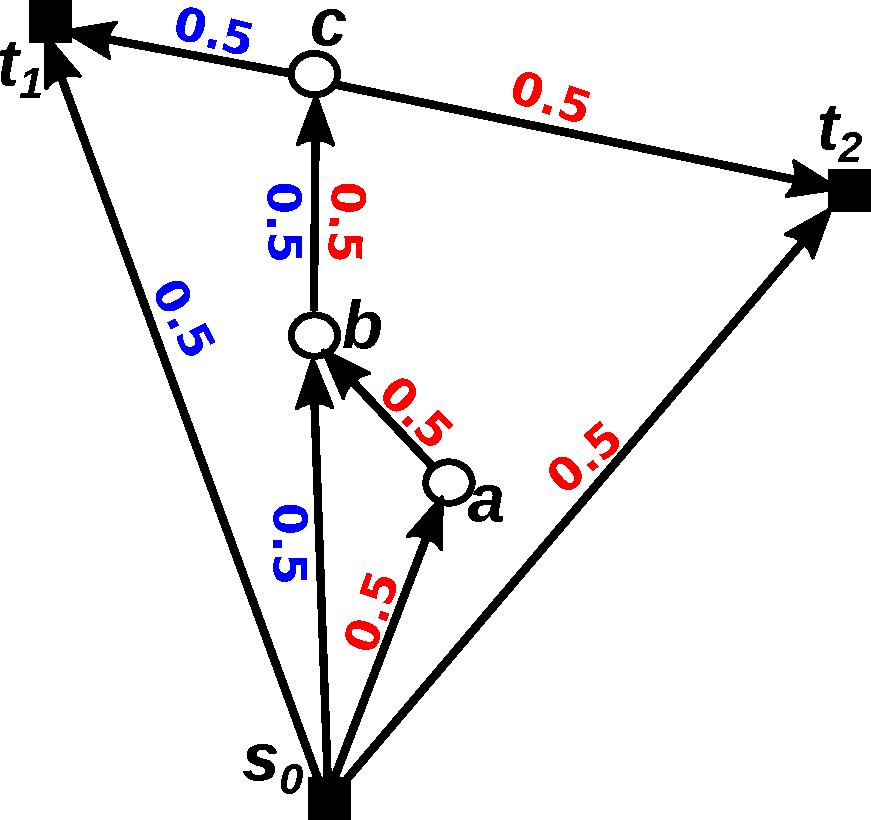
\includegraphics[height=2.3in]{counterex}
        \caption{A feasible solution to LP($\mathcal{F}_2$) of an instance on six vertices with destinations $D=\{s_0,t_1,t_2\}$.
		 Blue and red labels along the edges represent the amount of flow through a given edge towards $t_1$ and $t_2$, respectively.
		 In this solution, $g_{ij}>F^*_{ij}$, because if $x_{s_0i}=g_{ki}=0.
		5$, then $g_{ij}$ must be equal to 1 in order to fulfill (\ref{con:pf1:flowX}).}
        \label{fig:counterex}
\end{figure}
 
Consider an instance with optimal solution $(f,x,y)$ to LP($\mathcal{F}_2$) satisfying conditions in Lemma \ref{lem:onedir}.
If $(f,x,y)$ violates conditions in Lemma \ref{lem:oneslack}, it is possible to alter $x$ and obtain another optimum $(f,x',y)$ satisfying conditions in both lemmata \ref{lem:onedir} and \ref{lem:oneslack}.
Similarly, if $(f,x',y)$ still violates Lemma \ref{lem:xequals} at some arc $(i,j)$, the solution is altered by decreasing $x'_{ij}$ while preserving feasibility.
Once conditions in Lemma \ref{lem:onedir} and Lemma \ref{lem:oneslack} are satisfied, such a decrease cannot violate them.
These remarks are summarized as 
%%%%%%%%%%%%%%%%%%%%%%%%%%%%%%%%%%%%%%%
%                                     %
%         Observation 1               %
%                                     %
%%%%%%%%%%%%%%%%%%%%%%%%%%%%%%%%%%%%%%%
\begin{obs}
Instances of LP($\mathcal{F}_2$) have optimal solutions satisfying the conditions in all of Lemma \ref{lem:onedir}, Lemma \ref{lem:oneslack} and Lemma \ref{lem:xequals}.
\end{obs}
%%%%%%%%%%%%%%%%%%%%%%%%%%%%%%%%%%%%%%%
%                                     %
%         Proposition 2               %
%                                     %
%%%%%%%%%%%%%%%%%%%%%%%%%%%%%%%%%%%%%%%
\begin{prop}
\label{prop:f1strx2}
LP($\mathcal{F}_2$) is at least as strong as LP($\mathcal{X}_2$). 
\end{prop}
%%%%%%%%%%%%%%%%%%%%%%%%%%%%%%%%%%%%%%
%   Beginning of proof of Prop. 2    %
%%%%%%%%%%%%%%%%%%%%%%%%%%%%%%%%%%%%%%
\begin{proof}
Let (x,f,y) be an optimal solution to LP($\mathcal{F}_2$) satisfying the conditions in Lemmata \ref{lem:onedir}, \ref{lem:onedir} and \ref{lem:xequals}.
We show that each inequality in LP($\mathcal{X}_2$) is implied by inequalities in LP($\mathcal{F}_2$).

\begin{itemize}[leftmargin=1cm]
%\item[] (\ref{con:mfinpf2:maxsize}): Folaws directly from (\ref{eq:sumToD}) and (\ref{con:pf1:B}).
\item[ (\ref{con:mfinpf2:arrowFromDest}):] Assume $t\in D_0$ and $i\in D_0\setminus\{t\}$. Flow conservation (\ref{con:pf1:flow}) implies
	$$\sum_{j\in V_i}g_{ji} - \sum_{j\in V_i}F^t_{ji} + \sum_{j\in V_i}F^t_{ij} = \sum_{j\in V_i}g_{ji}.$$ Then (\ref{con:mfinpf2:arrowFromDest}) follows from Lemma \ref{lem:sumxji1}.
	Assume $i=s_0$. Due to (\ref{con:pf1:xi0=0}) and (\ref{con:pf1:xfrel}), the following first two sums equal zero, which gives
	$$\sum_{j\in V_i}g_{ji} - \sum_{j\in V_i}F^t_{ji} + \sum_{j\in V_i}F^t_{ij} = \sum_{j\in V_i}F^t_{ij} = 1,$$
	where the latter equality follows by summing (\ref{con:pf1:flow}) over all $i\in V\setminus\{s_0\}$. If $t=s_0$, then after applying definition (\ref{con:mfinpf2:fij00}), i. e., $F^0_{ij}=0$, (\ref{con:mfinpf2:arrowFromDest})  also follows from Lemma \ref{lem:sumxji1}. 
\item[ (\ref{con:mfinpf2:arrowFromNonDestB}):] The proof is analogous to (\ref{con:mfinpf2:arrowFromDest}), with (\ref{con:pf1:B}) replacing (\ref{eq:sumToD}).
\item[ (\ref{con:mfinpf2:arrowFromNonDestA}):] The inequality can be rewritten as
	\begin{align*}
	 g_{ij}  \leq& \sum\limits_{k \in V_i\setminus\{j\}}g_{ki}-\sum\limits_{k \in V_i\setminus\{j\}}F^s_{ki}+\sum\limits_{k \in V_i\setminus\{j\}}F^s_{ik} +F^s_{ij}-F^s_{ji} = \\
	 ~=& \sum\limits_{k \in V_i\setminus\{j\}}g_{ki}-\sum\limits_{k \in V_i}F^s_{ki}+\sum\limits_{k \in V_i}F^s_{ik} = \sum\limits_{k \in V_i\setminus\{j\}}g_{ki},
	\end{align*}
	where the last equality follows from the flow conservation (\ref{con:pf1:flow}). Now assume the contrary that for some $(i,j)\in A$, where $i\in V\setminus D$,
	\begin{align}
	g_{ij} > \sum\limits_{k \in V_i\setminus\{j\}}g_{ki}.\label{eq:assumContr}
	\end{align}
	The proof is divided into two parts that capture the two cases stated by Lemma \ref{lem:xequals}.
	Assume first that (L.4a) holds.
	We have that $\exists t\in D_0 \text{ s. t. }F^t_{ij}=g_{ij}$.
	Besides the strict inequality, assumption (\ref{eq:assumContr}) also implies $g_{ij}> 0$ which together with Lemma \ref{lem:onedir} gives $F^t_{ji}=0$.
 	By applying (\ref{con:pf1:xfrel}) to arcs entering $i$,
	$$\sum\limits_{k\in V_i}F^t_{ik} \geq F^t_{ij}=g_{ij}>\sum\limits_{k \in V_i\setminus\{j\}}g_{ki} \geq \sum\limits_{k \in V_i\setminus\{j\}}F^t_{ki}=\sum\limits_{k \in V_i}F^t_{ki},$$
	contradicting flow conservation constraints (\ref{con:pf1:flow}).
	Assume next that (L.4a) does not hold, i.e., $F^*_{ij}<g_{ij}$. 
	We know from Lemma \ref{lem:oneslack} that $g_{ji}=F^*_{ji}$, and so $\exists t\in D_0 \text{ s. t. }F^t_{ji}=g_{ji}$. 
	Moreover, Lemma \ref{lem:onedir} says that if for some $s\in D_0: F^s_{ji}>0$, then $F^s_{ij} = 0$, i.e. any flow that enters $i$ via $(j,i)$ must leave it through an arc different from $(i,j)$.
	Together with the flow conservation and (\ref{con:pf1:xfrel}),
	$$
	g_{ji}=F^t_{ji}\leq\sum_{k\in V_i}F^t_{ik}=\sum_{k\in V_i\setminus\{j\}}F^t_{ik}\leq\sum_{k\in V_i\setminus\{j\}}g_{ik}.
	$$
	Note that for $g_{ji}=F^t_{ji}=0$, $F^t_{ij}\geq 0$ in which case the second equality above would not hold, but we could directly write $g_{ji}\leq\sum_{k\in V_i\setminus\{j\}}g_{ik}$. 
	Combined with the assumption (\ref{eq:assumContr}) we obtain
	$$
	\sum_{k\in V_i}g_{ki} = g_{ji} + \sum_{k\in V_i\setminus\{j\}}g_{ki}<g_{ij} + \sum_{k\in V_i\setminus\{j\}}g_{ik} = \sum_{k\in V_i}g_{ik},
	$$
	contradicting (L.4b), and thereby Lemma \ref{lem:xequals}. 
	The proof applies with minor simplifications also for $s=s_0$.
\item[ (\ref{con:mfinpf2:startInSource}):] Follows from (\ref{con:pf1:noflowFromT}) and (\ref{con:pf1:fitt=xit}) if $s\in D_0$, or (\ref{con:pf1:xi0=0}) and (\ref{con:mfinpf2:fij00}) if $s=s_0$.
\item[ (\ref{con:mfinpf2:yvar}):] Identical to (\ref{con:pf1:yvar}) if $s\in D_0$, or follows from (\ref{con:pf1:yvar0}) and (\ref{con:mfinpf2:fij00}) if $s=s_0$.
\item[ (\ref{con:mfinpf2:extraCon}):] Follows immediately from (\ref{con:pf1:flowX}) by utilizing (\ref{con:pf1:flow}) at node $i$ if $s\in D_0$, or by utilizing (\ref{con:mfinpf2:fij00}) if $s=s_0$.
\item[(\ref{con:mfinpf2:sumYImpSumXTrans})] Follows from (\ref{con:vi:sumYImpSumXTrans}) by applying flow conservation at $i$ if $s\in D_0$, and by applying (\ref{con:mfinpf2:fij00}) if $s=s_0$. 
\item[(\ref{con:mfinpf2:flowNormal}):] All four-index variables cancel out. 
	Thus, (\ref{con:mfinpf2:flowNormal}) follows from flow conservation (\ref{con:pf1:flow}) at $i\in D_0$. and from (\ref{con:mfinpf2:fij00}) if $i=s_0$.
%\item[] (\ref{con:mfinpf2:fcap}): Follows from (\ref{con:pf2:stronger}).
\item[(\ref{con:mfinpf2:flowDest}):] Is implied by flow conservation at $t$  if $t\in D_0$. For $t=s_0$, by combining (\ref{con:mfinpf2:fij00}) and (\ref{con:pf1:xi0=0}) together with (\ref{con:pf1:xfrel}), we arrive at $\sum_{j\in V_0}F^s_{0j}=1$, which obviously (?) holds. 
\item[ (\ref{con:mfinpf2:zbound}):]
 	Adding $g_{ji}$ to (\ref{con:mfinpf2:arrowFromNonDestA}) gives the desired relation
	\[
	g_{ij}+g_{ji}\leq\sum_{k\in V_i\setminus\{j\}}g_{ki} +g_{ji}=\sum_{k\in V_i}g_{ki}\leq 1,
	\]
	where the last inequality follows from (\ref{con:pf1:B}) if $i\in V\setminus D$, and from Lemma \ref{lem:sumxji1} if $i\in D_0$. 
	Finally, if $i=s_0$, (\ref{con:mfinpf2:zbound}) is implied by combining (\ref{con:pf1:xi0=0}) together with relaxed integrality constraints.
	%It is sufficient to show this case for a non-destination $i$, because for $i\in D$,  $g_{ij}=F^*_{ij}$ would certainly hold, which is covered by the previous case. 
\item[ (\ref{con:mfinpf2:xbound}):] The lower bound follows from (\ref{con:pf1:xfrel}) for $s\in D_0$, and from (\ref{con:mfinpf2:fij00}) and non-negativity of $g_{ij}$ for $s=s_0$.
	The upper bound follows from (\ref{con:mfinpf2:arrowFromDest}) for $i\in D$ and from (\ref{con:mfinpf2:arrowFromNonDestB}) for $i\in V\setminus D$.
	To see this, observe that each term in the sums in (\ref{con:mfinpf2:arrowFromDest})-(\ref{con:mfinpf2:arrowFromNonDestB}) is non-negative because of (\ref{con:pf1:xfrel}).
\end{itemize}
Due to the symmetry $ f^{st}_{ij} =  f^{ts}_{ij}$, constraints (\ref{con:mfinpf2:fcap}) and (\ref{con:mfinpf2:fbound}) represent for each $(i,j)\in A$ and for each $\{s,t\}\in \check{S}_0$ relations
\begin{subequations}
\begin{align}
\label{fcapa} f^{st}_{ij} +  f^{st}_{ji} &\geq F^t_{ij} + F^s_{ij}-g_{ij}, \\
\label{fcapb} f^{st}_{ij} +  f^{st}_{ji} &\geq F^t_{ji} + F^s_{ji}-g_{ji}, \\
\label{fbounda}F^t_{ij}+ F^s_{ji}\geq f^{st}_{ij} +  f^{st}_{ji} &\geq F^t_{ji} + F^s_{ij}-1, \\
\label{fboundb}F^s_{ij}+ F^t_{ji}\geq f^{st}_{ij} +  f^{st}_{ji} &\geq F^s_{ji} + F^t_{ij}-1. 
\end{align}
\end{subequations}
From these inequalities,
$$
 F^{st}_{ij} +  F^{st}_{ji}\in\left[\max\{F^s_{ij}+F^t_{ji},F^t_{ij}+F^s_{ji}\}-1,\min\{F^s_{ij}+F^t_{ji},F^t_{ij}+F^s_{ji}\}\right].
$$
Assume without loss of generality that $F^s_{ij} + F^t_{ji}\leq F^t_{ij} + F^s_{ji}$. Assigning $ f^{st}_{ij}\coloneqq F^s_{ij}$ and $ f^{st}_{ji}\coloneqq F^t_{ji}$ does not violate any other constraint as the $ f$-variables appear only in (\ref{con:mfinpf2:fcap}) and (\ref{con:mfinpf2:fbound}).
\begin{itemize}[leftmargin=1cm]
\item[(\ref{con:mfinpf2:fcap}):]  Using $ f^{st}_{ij} +  f^{st}_{ji} = F^s_{ij} + F^{t}_{ji}$ and (\ref{con:mfinpf2:xbound}) we obtain inequalities
	\begin{align*}
	F^s_{ij} + F^{t}_{ji}-F^t_{ij}-F^s_{ij}+g_{ij}&\geq 0,\\
	F^s_{ij} + F^{t}_{ji}-F^t_{ji}-F^s_{ji}+g_{ij}&\geq 0,
	\end{align*}
	which shows that (\ref{fcapa}) and (\ref{fcapb}) hold under the selected values for $ f^{st}_{ij}$ and $ f^{st}_{ji}$.
\item[(\ref{con:mfinpf2:fbound}):] Again, from $ f^{st}_{ij} +  f^{st}_{ji} = F^s_{ij} + F^{t}_{ji}$  we get for (\ref{fbounda})
	\begin{align*}
	F^s_{ij} + F^{t}_{ji} + 1 &\geq F^s_{ij}+F^t_{ji},
	\end{align*}
	which obviously holds. Finally, utilizing (\ref{con:mfinpf2:xbound}) we obtain for (\ref{fboundb})
	\begin{align*}
	F^s_{ij} + F^{t}_{ji} + 1 -F^t_{ij}-F^s_{ji} &= F^s_{ij}-F^s_{ji}+F^t_{ji}-F^s_{ij}+1 \geq \\
	&\geq g_{ij}-1-g_{ij}+1=0.
	\end{align*}
%\item[] (\ref{con:mfinpf2:fbound}): The lower bound follows from (\ref{con:pf2:hookImpFs})-(\ref{con:pf2:hookImpFt}). From (\ref{eq:fimpx}) and (\ref{con:mfinpf2:zbound}), we get the upper bound
%$$F^t_{ij}+F^s_{ji}-f^{st}_{ij}-f^{st}_{ji}\leq F^t_{ij}+F^s_{ji}\leq g_{ij}+g_{ji}\leq 1$$
\end{itemize}\qed
\end{proof} 
%%%%%%%%%%%%%%%%%%%%%%%%%%%%%%%%%%%%%%
%   End of proof of Prop. 2          %
%%%%%%%%%%%%%%%%%%%%%%%%%%%%%%%%%%%%%%
Note that in parts (\ref{con:mfinpf2:arrowFromNonDestA}) and (\ref{con:mfinpf2:xbound}) of this proof it is necessary to assume $\mathcal{F}_1$ instead of $\mathcal{F}_2$.
The arguments work with (\ref{con:pf1:xfrel}), but could not be used with stronger (\ref{con:pf2:stronger}).
Proposition \ref{prop:f1strx2} suggests that additional 4-index variables in $\mathcal{X}_2$ model are not very beneficial, because the formulation is implied by the smaller $\mathcal{F}_2$.
Nonetheless, introducing $\mathcal{X}_2$ is justified because of valid inequalities (\ref{con:vi:f2dest})-(\ref{con:vi:sumFImpSumY}) that significantly strengthen the model and can also be converted into $\mathcal{F}_2$ space and also increase the LP bound.

%%%%%%%%%%%%%%%%%%%%%%%%%%%%%%%%%%%%%%%
%                                     %
%         Proposition 3               %
%                                     %
%%%%%%%%%%%%%%%%%%%%%%%%%%%%%%%%%%%%%%%
\begin{prop}
\label{prop:x2strf1}
LP($\mathcal{X}_2$) is at least as strong as LP($\mathcal{F}_2$). 
\end{prop}
\begin{proof}
The approach is analogous the the proof of Proposition \ref{prop:f1strx2}.
We express $\mathcal{F}_2$ in the space of $\mathcal{X}_2$ using transformations (\ref{eq:tr:xij=xij0}) and (\ref{eq:tr:fijt2}).
After applying these transformations on (\ref{con:pf1:xfrel}), (\ref{con:pf1:flow}), (\ref{con:pf1:yvar0}), (\ref{con:pf1:B}), (\ref{con:pf1:xi0=0}), (\ref{con:pf1:dim}) and (\ref{con:pf1:flowX}), we immediately obtain constraints already present in $\mathcal{X}_2$.
Similarly, applying transformation (\ref{eq:tr:xijj}) on constraints (\ref{con:pf1:yvar}) and (\ref{con:vi:sumYImpSumXTrans}) results in (\ref{con:dd:yvar}) and (\ref{con:vi:sumYImpSumX}).
For (\ref{con:pf1:noflowFromT}) we get $F^t_{ti}=f^{0t}_{ti}=f^{t0}_{it}\leq x^t_{it}=0$ by utilizing (\ref{con:mf:fsym}) and (\ref{con:mfinpf2:fcap}).
Finally, we have $$1=\sum_{i\in V_t}f^{0t}_{it}\leq \sum_{i\in V_t}x^0_{it}=1,$$ where the first equality follows from (\ref{con:mf:flowDest}) and already proved $f^{0t}_{ti}=0, t\in D_0,i\in V_t$, and the second equality is a part of (\ref{con:dd:arrowFromDest}).
The inequality is a consequence of (\ref{con:mf:fcap}), but clearly it must be satisfied with equality, and thus individual corresponding summands must be equal too.
 
\qed
\end{proof}
The combination of Propositions \ref{prop:f1strx2} and \ref{prop:x2strf1} implies
%%%%%%%%%%%%%%%%%%%%%%%%%%%%%%%%%%%%%%%
%                                     %
%         Corollary 1                 %
%                                     %
%%%%%%%%%%%%%%%%%%%%%%%%%%%%%%%%%%%%%%%
\begin{corollary}
Models $\mathcal{X}_2$ and $\mathcal{F}_2$ are equally strong.
\end{corollary}

\section{Constraint Generation Scheme}
\label{sec:cg}
Owing to the large number of constraints in the stronger models, LP($\mathcal{X}_3$) and LP($\mathcal{F}_3$) are impractical for computing lower bounds, even in fairly small instances.
The main idea of how to tackle larger instances and thereby make these models more useful in practice is to solve a relaxation of the model where some of the constraints are omitted.
It is assumed that the omitted constraints are often satisfied in solution of the relaxed problem, without being explicitly included in the model.
Relaxed constraints that are violated in the obtained solutions can be dynamically added to the model and the whole process is repeated, until some termination criteria are fulfilled.
This approach is known as a \emph{constraint generation scheme}.

\subsection{Implementation}%

%Experimental evaluation from the next section reveals that the valid inequality (\ref{con:vi:sumFImpSumY}) makes $\mathcal{X}_3$ very strong, in fact its LP relaxation often gives an integral solution.
%To the contrary, the other valid inequalities (\ref{con:vi:f2dest}) and (\ref{con:vi:xImpSumF}) rarely improve the LP bounds, and moreover increase the runtime.
For these practical reasons, we consider the model X2+(\ref{con:vi:sumFImpSumY}) for constraint generation.
Also note that LP($\mathcal{X}_1$) has the shortest runtime but not much shorter than LP($\mathcal{X}_2$).
The idea is therefore to solve LP($\mathcal{X}_2$) and generate only those remaining constraints that are violated.

For each $(s,t)\in S$, constraints (\ref{con:mf:flowNormal})-(\ref{con:mf:fcap})form a classical maximum flow formulation which can be solved very quickly.
Observe that according to (\ref{con:mf:fcap}), $x^s$ plays the role of a capacity vector in the network $G_{x^s}=(V,E,s,t,x^s)$ in which we want to find the maximum flow, and thereby verify whether the flow conservation constraints are already satisfied even though they are not explicitly included in the model.
The formulation can also be extended by (\ref{con:vi:sumFImpSumY}).
Unfortunately, including (\ref{con:mf:fsym}) is slightly problematic here, because it contains variables of a different commodity, namely $(t,s)$.
It is not possible to simply extend the model by these constraints, because a potential violation of flow conservation for the commodity $(t,s)$ would not be discovered, as there are no corresponding capacity constraints.
Nevertheless, this can be easily resolved by combining the two commodities in one maximum flow formulation.
As $s$ and $t$ are now constants, let $f_{ij}=f^{st}_{ij}$.

This extended maximum flow formulation denoted as 2MF is constructed as follows:
\newline
\newline  
%%%%%%%%%%%%%%%%%%%%%%%%%%%%%%%%%%%%%%%
%                                     %
%          Model 2MF                  %
%        (13a) - (13f)                %
%                                     %
%%%%%%%%%%%%%%%%%%%%%%%%%%%%%%%%%%%%%%%
\begin{subequations}\label{eq:mf}
\begin{align}
\label{objective:maxf} &\max\sum\limits_{i \in V_s} f_{si} \\ 
\text{s.t.}  \notag   \\
\label{con:maxf:flowNormal}  \sum\limits_{\substack{ j\in V_i}}\left(f_{ij}-f_{ji}\right) & = 0 & i\in V\setminus\{s,t\},\\
\label{con:maxf:fcapst}   f_{ij} &\leq \min\{X_{ij}^s, X_{ji}^t\}     &  (i,j)\in A,  \\ 	 
\label{con:maxf:sumFImpSumYst} \sum\limits_{k\in V_i:p_{ik}\geq p_{ij}}f_{ik} & \leq \sum\limits_{k\in V_i:p_{ik}\geq p_{ij}}  \pi^{s}_{ik} & i,j\in V,\\
\label{con:maxf:sumFImpSumYts} \sum\limits_{k\in V_i:p_{ik}\geq p_{ij}}f_{ki} & \leq \sum\limits_{k\in V_i:p_{ik}\geq p_{ij}}  \pi^{t}_{ik} &  i,j\in V,\\
\label{con:maxf:fdim}f&\in\left[0,1\right]^{A}. 
\end{align}~
\end{subequations}  
  
This model comprises of constraints for $\{s,t\}\in\check{S}$ that are in $\mathcal{X}_3$ but not in $\mathcal{X}_2$.
Note that the right-hand sides in (\ref{con:maxf:fcapst})-(\ref{con:maxf:sumFImpSumYts}) are not variables.
These values are input data obtained by solving LP($\mathcal{X}_2$).
The problem modelled by this formulation can be understood as a maximum 2-commodity network flow, where the source of the first commodity is the target of the second commodity and vice versa.
Furthermore, the arcs have different capacities for the two commodities, even though it is required that the amount of one commodity passing through an arc $(i,j)$ equals the amount of the other commodity passing through $(j,i)$.
Due to the flow symmetry (\ref{con:mf:fsym}), we can always substitute $f^{ts}_{ji}$ with $f^{st}_{ij}$, and it is done so in (\ref{con:maxf:fcapst}) and (\ref{con:maxf:sumFImpSumYts}).
 
Based on these observations we build the constraint generation procedure.
First, we solve LP($\mathcal{X}_2$) and obtain vectors $x$ and $y$.
For each $(s,t)\in \check{S}$ we then check whether the relaxed constraints (\ref{con:mf:flowNormal})-(\ref{con:mf:fsym}) together with (\ref{con:vi:sumFImpSumY}) can already be satisfied by solving 2MF.
In case the objective value is 1, the relaxed constraints are satisfied.
Otherwise, we record the pair $(s,t)$, and after processing all pairs, relaxed constraints for a selection of the recorded pairs are added to the original model.
This augmented model is then solved again yielding new input values for the next iteration of the verification by 2MF.
The whole process is repeated until there are no violated flow constraints for any $(s,t)$ pair.
Algorithm \ref{alg:cg} describes the process more formally.

%%%%%%%%%%%%%%%%%%%%%%%%%%%%%%%%%%%%%%%
%                                     %
%         Algorithm 1                 %
%                                     %
%%%%%%%%%%%%%%%%%%%%%%%%%%%%%%%%%%%%%%%
\begin{algorithm}
\KwData{SMT instance}
\KwResult{Solution to LP($\mathcal{X}_3$)}
$Q'\leftarrow\emptyset$\tcp*{$\{s,t\}$ pairs of which constraints are to be added to $\mathcal{X}_2$}
\Do {$Q'\neq\emptyset$}{
	$Q\leftarrow\emptyset$\tcp*{Violated $\{s,t\}$ pairs} 
	\tcc{Solve the instance using $\mathcal{X}_2$ extended by constraints from 2MF associated with $\{s,t\}$ pairs in $Q'$}
	$(x,y)\leftarrow\text{solve($\mathcal{X}_2$,$Q'$.)}$\;
	\For{$\{s,t\}\in \check{S}$} {
		\tcc{Find the objective value of the extended maximum flow problem instance for given commodity $(s,t)$ using the capacities obtained earlier.}
		$v^*\leftarrow \text{solve(2MF,$s$,$t$,$x$,$y$)}$\;
		\If{$v^* < 1$} {
			$ Q\leftarrow Q\cup \{\{s,t\}\}$\;
		}
	}
	Select some subset $Q'\subseteq Q$ of the violated $\{s,t\}$ pairs according to a given strategy where $Q'\neq\emptyset$ if $Q\neq\emptyset$.
}
 ~\newline
 \caption{Constraint generation}
\label{alg:cg}
\end{algorithm}

\subsection{Strategies for constraint generation}

There are various strategies for selection of the violated flow constraints to be added to the original model.
Here are described those that we consider in the experimental part of this work.

\subsubsection{Add all}

One of the most basic strategies adds constraints of all violated $\{s,t\}$ pairs.
This approach turns out to be less practical, because after the first iteration, most of the $\{s,t\}$ pairs violate the 2MF constraints, and we end up adding too many of them which usually leads to a very long runtime of the next iteration.

\subsubsection{Add the first $k$}

Another simple strategy adds the first $k$ found $\{s,t\}$ pairs violating the flow constraints.
Even though it is not necessary to solve 2MF for all possible pairs of destinations, the runtime does not decrease noticeably.
Like in the previous case, this strategy does not exploit the structure of the graph induced by the violated $\{s,t\}$ pairs in any way.

\subsubsection{Add the best $k$}

This strategy is based on the assumption that addition of constraints for $\{s,t\}$ pairs for which the maximum flow value is lower, and are thus "more violated", is more likely to cause satisfaction of a larger number of constraints associated with other pairs of destinations that are violated but not yet included in $Q'$.

\subsubsection{Add maximum matching}

Another assumption that can be made is that addition of constraints for a given $\{s,t\}$ is likely to cause satisfaction of constraints associated with an adjacent pair $\{t,u\}$.
Thus, we are looking for a (maximum) matching $M$ in the weighted graph $(D,\check{S},w)$, where the weight function $w:\check{S}\to\mathbb{R}$ can be defined in several ways.
Probably the most intuitive is to use $v^*$ from Alg. \ref{alg:cg}.
Another suggestion is to define $w(\{s,t\})=p_{st}$, which is based on the assumption that a path between two distant nodes is long and addition of associated constraints may affect more edges.

%
%subsubsection{Add maximum spanning tree}
%
%\subsubsection{Heuristics}
%

\section{Experimental Evaluation}
\label{sec:exp}

The practical part of this work focuses on comparison of the models presented in the previous section.
As the main goal of this study is to determine tighter bounds, the conducted experiments are designed for this purpose.
Instances of intended number of vertices are generated with random coordinates uniformly distributed between [0, 0] and [100, 100].
All computations were made on an Intel Core 2 Quad CPU at 2.83 GHz and 8 GB RAM.
The models were implemented in Java with Concert technology and solved using CPLEX 12.5.1 optimizer.
 
%\subsection{Instance generation}
\subsection{Comparison of the models}

The first experimental settings gives an overview of the studied models with respect to their strength and computational time.

\begin{table}[h!]
\centering
\setlength{\tabcolsep}{6pt} % Default value: 6pt
\renewcommand{\arraystretch}{1.4} % Default value: 1
\begin{tabular}{rrrrrrrr}
$|V|$ & $|D|$ & $LP(\mathcal{X}_1)$ & $LP(\mathcal{F}_1)$ & $LP(\mathcal{X}_2)$ & $LP(\mathcal{F}_2)$ & $LP(\mathcal{X}_3)$ &$LP(\mathcal{F}_3)$\\\hline
  16 & 8       & 72.25  & 80.39  & 82.20    & 85.97    & 99.78  & 99.78\\
  18 & 9       & 65.68  & 77.17  & 74.48    & 79.84    & 99.70  & 74.17\\ 
\end{tabular}
\caption{Average proportion of the optimal value calculated from 25 instances}
\label{tab:small_inst_cost}
\end{table}

\begin{table}[h!]
\centering
\setlength{\tabcolsep}{6pt} % Default value: 6pt
\renewcommand{\arraystretch}{1.4} % Default value: 1
\begin{tabular}{rrrrrrrrr}
 $|V|$ & $|D|$ & $LP(\mathcal{X}_1)$ & $LP(\mathcal{F}_1)$ & $LP(\mathcal{X}_2)$ & $LP(\mathcal{F}_2)$ & $LP(\mathcal{X}_3)$ & $LP(\mathcal{F}_3)$ & $\mathcal{F}_1$\\ \hline
  16 & 8       & 1   & 1   & 1     & 1     & 72  & 304  & 18 \\
  18 & 9       & 1   & 2   & 2     & 2     & 326 & 1140 & 65 \\ 
\end{tabular}
\caption{Comparison of average runtime in seconds}
\label{tab:small_inst_time}
\end{table}

\subsection{Experiments on small instances}

Small instances can often be solved to optimality relatively quickly with branch and bound (B\&B).
We investigate what is the maximum size of instances that can be solved to optimality within 20 minutes using models $\mathcal{X}_1$ and $\mathcal{F}_1$.
The experiments compare sets of instances with different $|V|/|D|$ ratio.
Each value in Tab. \ref{tab:small_inst} was obtained after solving 25 instances with given numbers of destinations and non-destinations.
 
\begin{table}[h!]
\centering
\setlength{\tabcolsep}{12pt} % Default value: 6pt
\renewcommand{\arraystretch}{1.4} % Default value: 1
\begin{tabular}{rrrrrrrr}
  ~ & ~ & \multicolumn{2}{c}{average time [s]} &\multicolumn{2}{c}{\# solved} &\multicolumn{2}{c}{\shortstack{average \\remaining gap[\%]}}\\ \hline
 $|V|$ & $|D|$ & $\mathcal{F}_1$   & $\mathcal{X}_1$   & $\mathcal{F}_1$ & $\mathcal{X}_1$ & $\mathcal{F}_1$ & $\mathcal{X}_1$\\ \hline
  18 & 12      & 84   & 139  & 25 & 24 & 0.00  & 0.52\\
  21 & 14      & 789  & 1006 & 18 & 10 & 5.08  & 9.64\\ 
  24 & 16      & 1137 & 1161 & 4  & 3  & 20.52 & 21.04\\ \hline 
 %27 & 18 & ~ & ~ & ~ & ~ & ~ & ~\\  
 20 & 10 & 190 & 387 & 25 & 21 & 0.00 & 3.00 \\
  22 & 11 & 637 & 880 & 22 & 14 & 0.64 & 7.16\\
  24 & 12 & 997 & 1169 & 10 & 3 & 10.44 & 16.44\\ \hline
 % 26 & 13 & 1189 & 1200 & 1 & 0 & ~ & ~\\ \hline
  21 & 7 & 113 & 282 & 25 & 21 & 0.00 & 2.56\\ 
  24 & 8 & 442 & 650 & 21 & 16 & 2.72 & 8.64\\ 
  27 & 9 & 1013 & 1146 & 8 & 4 & 14.64 & 22.80\\ 
\end{tabular}
\caption{Computational results of Branch and bound on small instances}
\label{tab:small_inst}
\end{table}

\subsection{Experiments on medium size instances}

When it is not possible to solve integer models within the given time limit, we pursue lower bounds obtained by solving LP relaxations of the models.
We want to get as strong lower bound as possible, but as shown in the previous sections, LP relaxations of the strongest models have worse runtime than basic IP models, and at this point the constraint generation scheme comes into play.
Using this method, it is possible to get strong lower bounds quickly, often even an integral solution.

B\&B also produces LP relaxation during its course, and even though the computation is interrupted before the optimum is found, it is possible to keep track of the best bound at any moment of the computation.
We compare the progress of objective value obtained by the CG method and the best lower bound found by applying B\&B to $\mathcal{F}_1$ a restricted amount of time.
 
The values in the graphs represent a mean percentage of an objective value yielded by LP($\mathcal{F}_1$).
The values are calculated from 5 instances.
 
\begin{figure}[!htb]
    \centering
    \begin{subfigure}[b]{0.49\textwidth}
        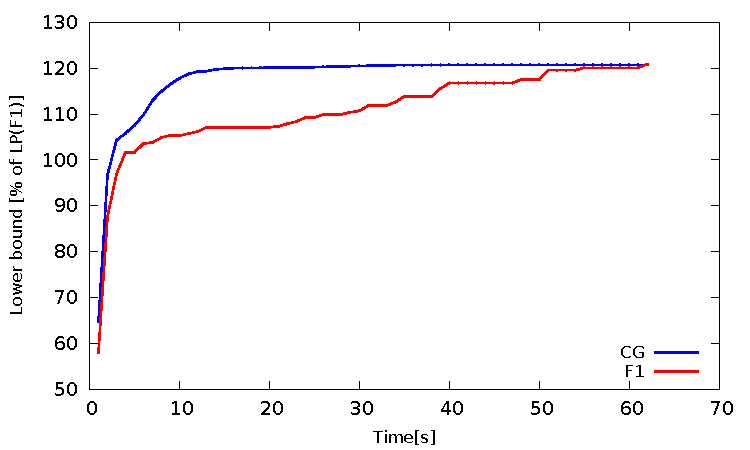
\includegraphics[width=\textwidth]{lower-bound-18-9}
        \caption{$|V|=18, |D|=9$}
        \label{fig:cggr18-9}
    \end{subfigure}
    \hfill %add desired spacing between images, e. g. ~, \quad, \qquad, \hfill etc. 
      %(or a blank line to force the subfigure onto a new line)
    \begin{subfigure}[b]{0.49\textwidth}
        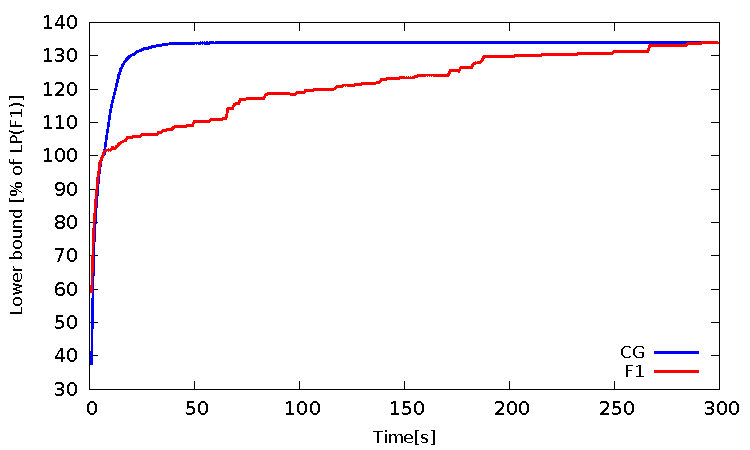
\includegraphics[width=\textwidth]{lower-bound-20-10}
        \caption{$|V|=20, |D|=10$}
        \label{fig:cggr20-10}
    \end{subfigure}
  
    \begin{subfigure}[b]{0.49\textwidth}
        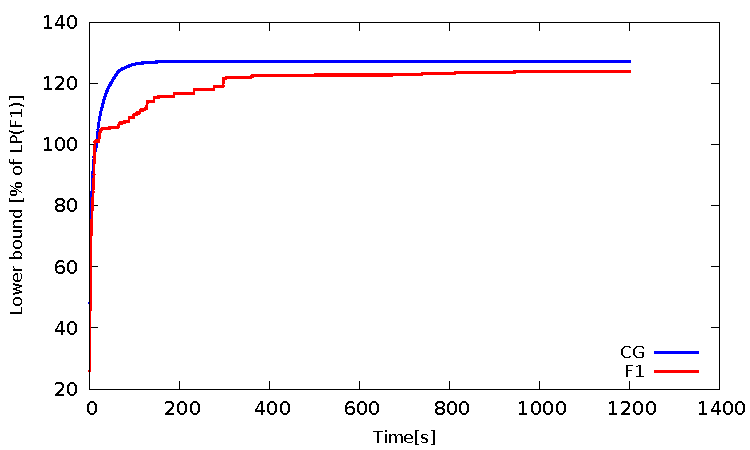
\includegraphics[width=\textwidth]{lower-bound-22-11}
        \caption{$|V|=22, |D|=11$}
        \label{fig:cggr22-11}
    \end{subfigure}
    \hfill %add desired spacing between images, e. g. ~, \quad, \qquad, \hfill etc. 
      %(or a blank line to force the subfigure onto a new line)
    \begin{subfigure}[b]{0.49\textwidth}
        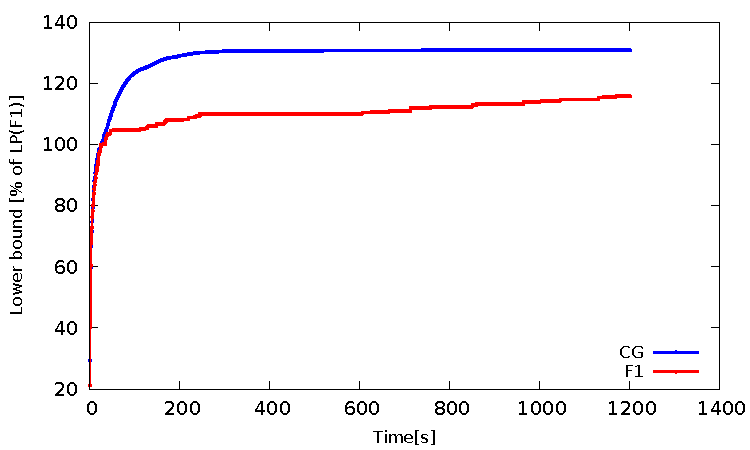
\includegraphics[width=\textwidth]{lower-bound-24-12}
        \caption{$|V|=24, |D|=13$}
        \label{fig:cggr24-12}
    \end{subfigure}

    \begin{subfigure}[b]{0.49\textwidth}
        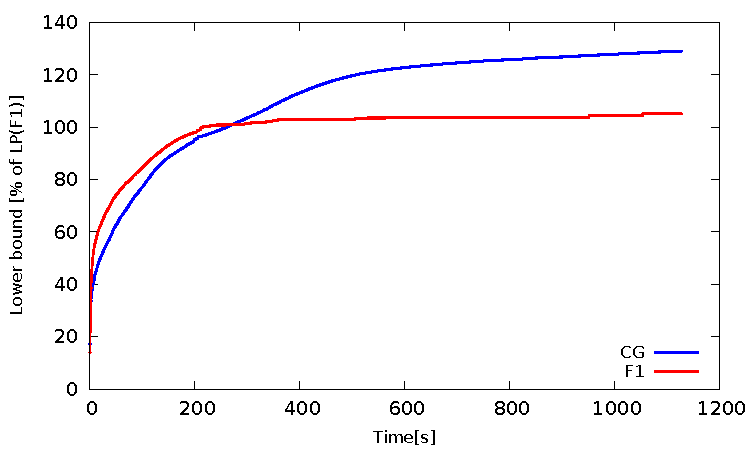
\includegraphics[width=\textwidth]{lower-bound-30-15}
        \caption{$|V|=30, |D|=15$}
        \label{fig:cggr30-15}
    \end{subfigure}
    \hfill %add desired spacing between images, e. g. ~, \quad, \qquad, \hfill etc. 
      %(or a blank line to force the subfigure onto a new line)
    \begin{subfigure}[b]{0.49\textwidth}
        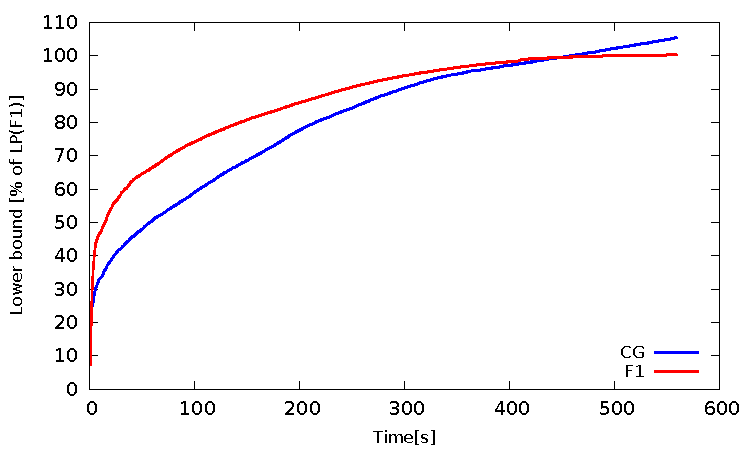
\includegraphics[width=\textwidth]{lower-bound-32-16}
        \caption{$|V|=32, |D|=16$}
        \label{fig:cggr32-16}
    \end{subfigure}
  \caption{Comparison of lower bound obtained by constraint generation and branch and bound on model $\mathcal{F}_1$. } \label{fig:cggr}
\end{figure} 

It is clear from the graphs that constraint generation is a suitable method for obtaining a lower bound for instances that cannot be solved to optimality using B\&B. CG provides a tighter bound at any time step of the computation.

\subsection{Experiments on large instances}

For instances in which $\mathcal{X}_3$ cannot be solved by CG within the given time limit, we investigate the best lower bounds that can be achieved by solving the LP relaxations of the weaker models.

\section{Conclusion and Future Work}
\label{sec:conclusion}


%as required. Don't forget to give each section
%and subsection a unique label (see Sect.~\ref{sec:1}).
%\paragraph{Paragraph headings} Use paragraph headings as needed.
%\begin{equation}
%a^2+b^2=c^2
%\end{equation}

% For one-column wide figures use
%\begin{figure}
% Use the relevant command to insert your figure file.
% For example, with the graphicx package use
%  \includegraphics{example.eps}
% figure caption is below the figure
%\caption{Please write your figure caption here}
%\label{fig:1}       % Give a unique label
%\end{figure}
%
% For two-column wide figures use
%\begin{figure*}
% Use the relevant command to insert your figure file.
% For example, with the graphicx package use
%  \includegraphics[width=0.75\textwidth]{example.eps}
% figure caption is below the figure
%\caption{Please write your figure caption here}
%\label{fig:2}       % Give a unique label
%\end{figure*}
%
% For tables use
%\begin{table}
% table caption is above the table
%\caption{Please write your table caption here}
%\label{tab:1}       % Give a unique label
% For LaTeX tables use
%\begin{tabular}{lll}
%\hline\noalign{\smallskip}
%first & second & third  \\
%\noalign{\smallskip}\hline\noalign{\smallskip}
%number & number & number \\
%number & number & number \\
%\noalign{\smallskip}\hline
%\end{tabular}
%\end{table}


%\begin{acknowledgements}
%If you'd like to thank anyone, place your comments here
%and remove the percent signs.
%\end{acknowledgements}

% BibTeX users please use one of
%\bibliographystyle{spbasic}      % basic style, author-year citations
%\bibliographystyle{spmpsci}      % mathematics and physical sciences
%\bibliographystyle{spphys}       % APS-like style for physics
%\bibliography{}   % name your BibTeX data base

% Non-BibTeX users please use
\begin{thebibliography}{}

%
% and use \bibitem to create references. Consult the Instructions
% for authors for reference list style.
%
\bibitem{Wieseltier00onthe}
Wieselthier,  J. E., Nguyen, G. D., Ephremides, A.,
On the Construction of Energy-Efficient Broadcast and Multicast Trees in Wireless Networks,
Proceedings of the Nineteenth Annual Joint Conference of the IEEE Computer and Communications Societies.
2, 585--594 (2000)

\bibitem{Haugland12Dual}
Yuan, D., Haugland, D.,
Dual Decomposition for Computational Optimization of Minimum-Power Shared Broadcast Tree in Wireless Networks,
IEEE Transactions on Mobile Computing,
12, 11, 2008--2019 (2012)

\bibitem{Polzin}
Polzin, T., Daneshmand, S. V., A comparison of Steiner tree relaxations, Discrete Applied Mathematics, 112,  1-3, 15 241--261, (2001)

\bibitem{ivanova16isco}
Ivanova, M., Shared Multicast Trees in Ad Hoc Wireless Networks, Combinatorial Optimization, 4th International Symposium, ISCO 2016, 241--261, (2016)

\bibitem{Haugland11Compact}
Haugland, D., Yuan, D.,
Wireless Network Design: Optimization Models and Solution Procedure, 219--246,
International Series in Operations Research \& Management Science.
Springer, New York, (2011)

\bibitem{Papadimitriou06SBT}
Papadimitriou, I., and Georgiadis, L.:
Minimum-energy Broadcasting in Multi-hop Wireless Networks Using a Single Broadcast Tree.
Mobile Networks and Applications.
11, 3, 361--375 (2006)

\bibitem{goemans93catalog}
Goemans, M. X., Myung, Y-S.,
A catalog of steiner tree formulations, 
Networks.
23, 1, 19--28 (1993) 

\bibitem{diane93ipf}
Dian{\'e}, M., Plesn{\'i}k, J.,
An integer programming formulation of the Steiner problem in graphs,
Zeitschrift f{\"u}r Operations Research.
37, 1, 107--111 (1993)

%\bibitem{RefJ}
% Format for Journal Reference
%Author, Article title, Journal, Volume, page numbers (year)
% Format for books
%\bibitem{RefB}
%Author, Book title, page numbers. Publisher, place (year)
% etc
\end{thebibliography}

\end{document}
% end of file template.tex

